% !TeX spellcheck = it_IT
\documentclass[11pt, twocolumn]{article}

\usepackage{graphicx}
\usepackage{enumitem}
\usepackage[dvipsnames]{xcolor}

\newenvironment{myitemize}
{ \begin{itemize}[topsep=0ex]
		\setlength{\itemsep}{0pt}
		\setlength{\parskip}{0pt}
		\setlength{\parsep}{0pt}     }
	{ \end{itemize}                  } 

\newenvironment{myenumerate}
{ \begin{enumerate}[topsep=0ex]
		\setlength{\itemsep}{0pt}
		\setlength{\parskip}{0pt}
		\setlength{\parsep}{0pt}     }
	{ \end{enumerate}                  } 


\title{Technological Infrastructures}
\author{}
\date{}

\begin{document}

\maketitle

%\begin{abstract}
%L'obiettivo del corso è forninre conoscenza solida delle piattaforme tecnologiche e computing platforms.
%Differenza delle responsabilità di Data Scientist e Data Engineer.
%Il corso è diviso in 2 parti.
%L'esame consiste in 15 domande sia aperte che chiuse per parte e si può arrivare a 30 con lo scritto, si può fare un progetto non obbligatorio che vale al più 3 punti.
%\end{abstract}

\part*{Part I - Prof Ciavotta}

\section{Componenti di NIST}
NIST sviluppa standard di riferimento per il pubblico. Software Architecture è un organizzazione globale di sistemi software, e consiste in:
\begin{myitemize}
	\item Divisione della componenti software in sottosistemi; 
	\item Definizione delle politiche con cui questi sistemi interagiscono;
	\item Definizione delle interfacce tra le varie componenti.
\end{myitemize}
Un'architettura di riferimento è essenzialmente un template (scatola vuota con elementi prefissati), fornisce solo il vocabolario usato comunemente per discutere le implementazioni di un dato software.\\
Un'architettura di riferimento per il software non è altro che architettura software dove le strutture e i vari elementi e relazioni sono forniti dai template.
\\
L'architettura di riferimento, fornita da NIST, per i Big Data:
\begin{myitemize}
	\item Fornisce un linguaggio comune per i stakeholders;
	\item Incoraggia aderenza ai standard comuni;
	\item Permette di implementare le architetture con una certa consistenza;
	\item Illustra e migliora la comprensione delle componenti, processi e  sistemi di Big Data;
\end{myitemize}

\subsection{I 5 ruoli principali per Big Data}
L'architettura concettuale dei Big Data è un architettura a croce con due assi: Information value (IV) e Information Technology (IT) (Fig \ref{fig:NBDRA}).\\
\begin{figure*}
	\centering
	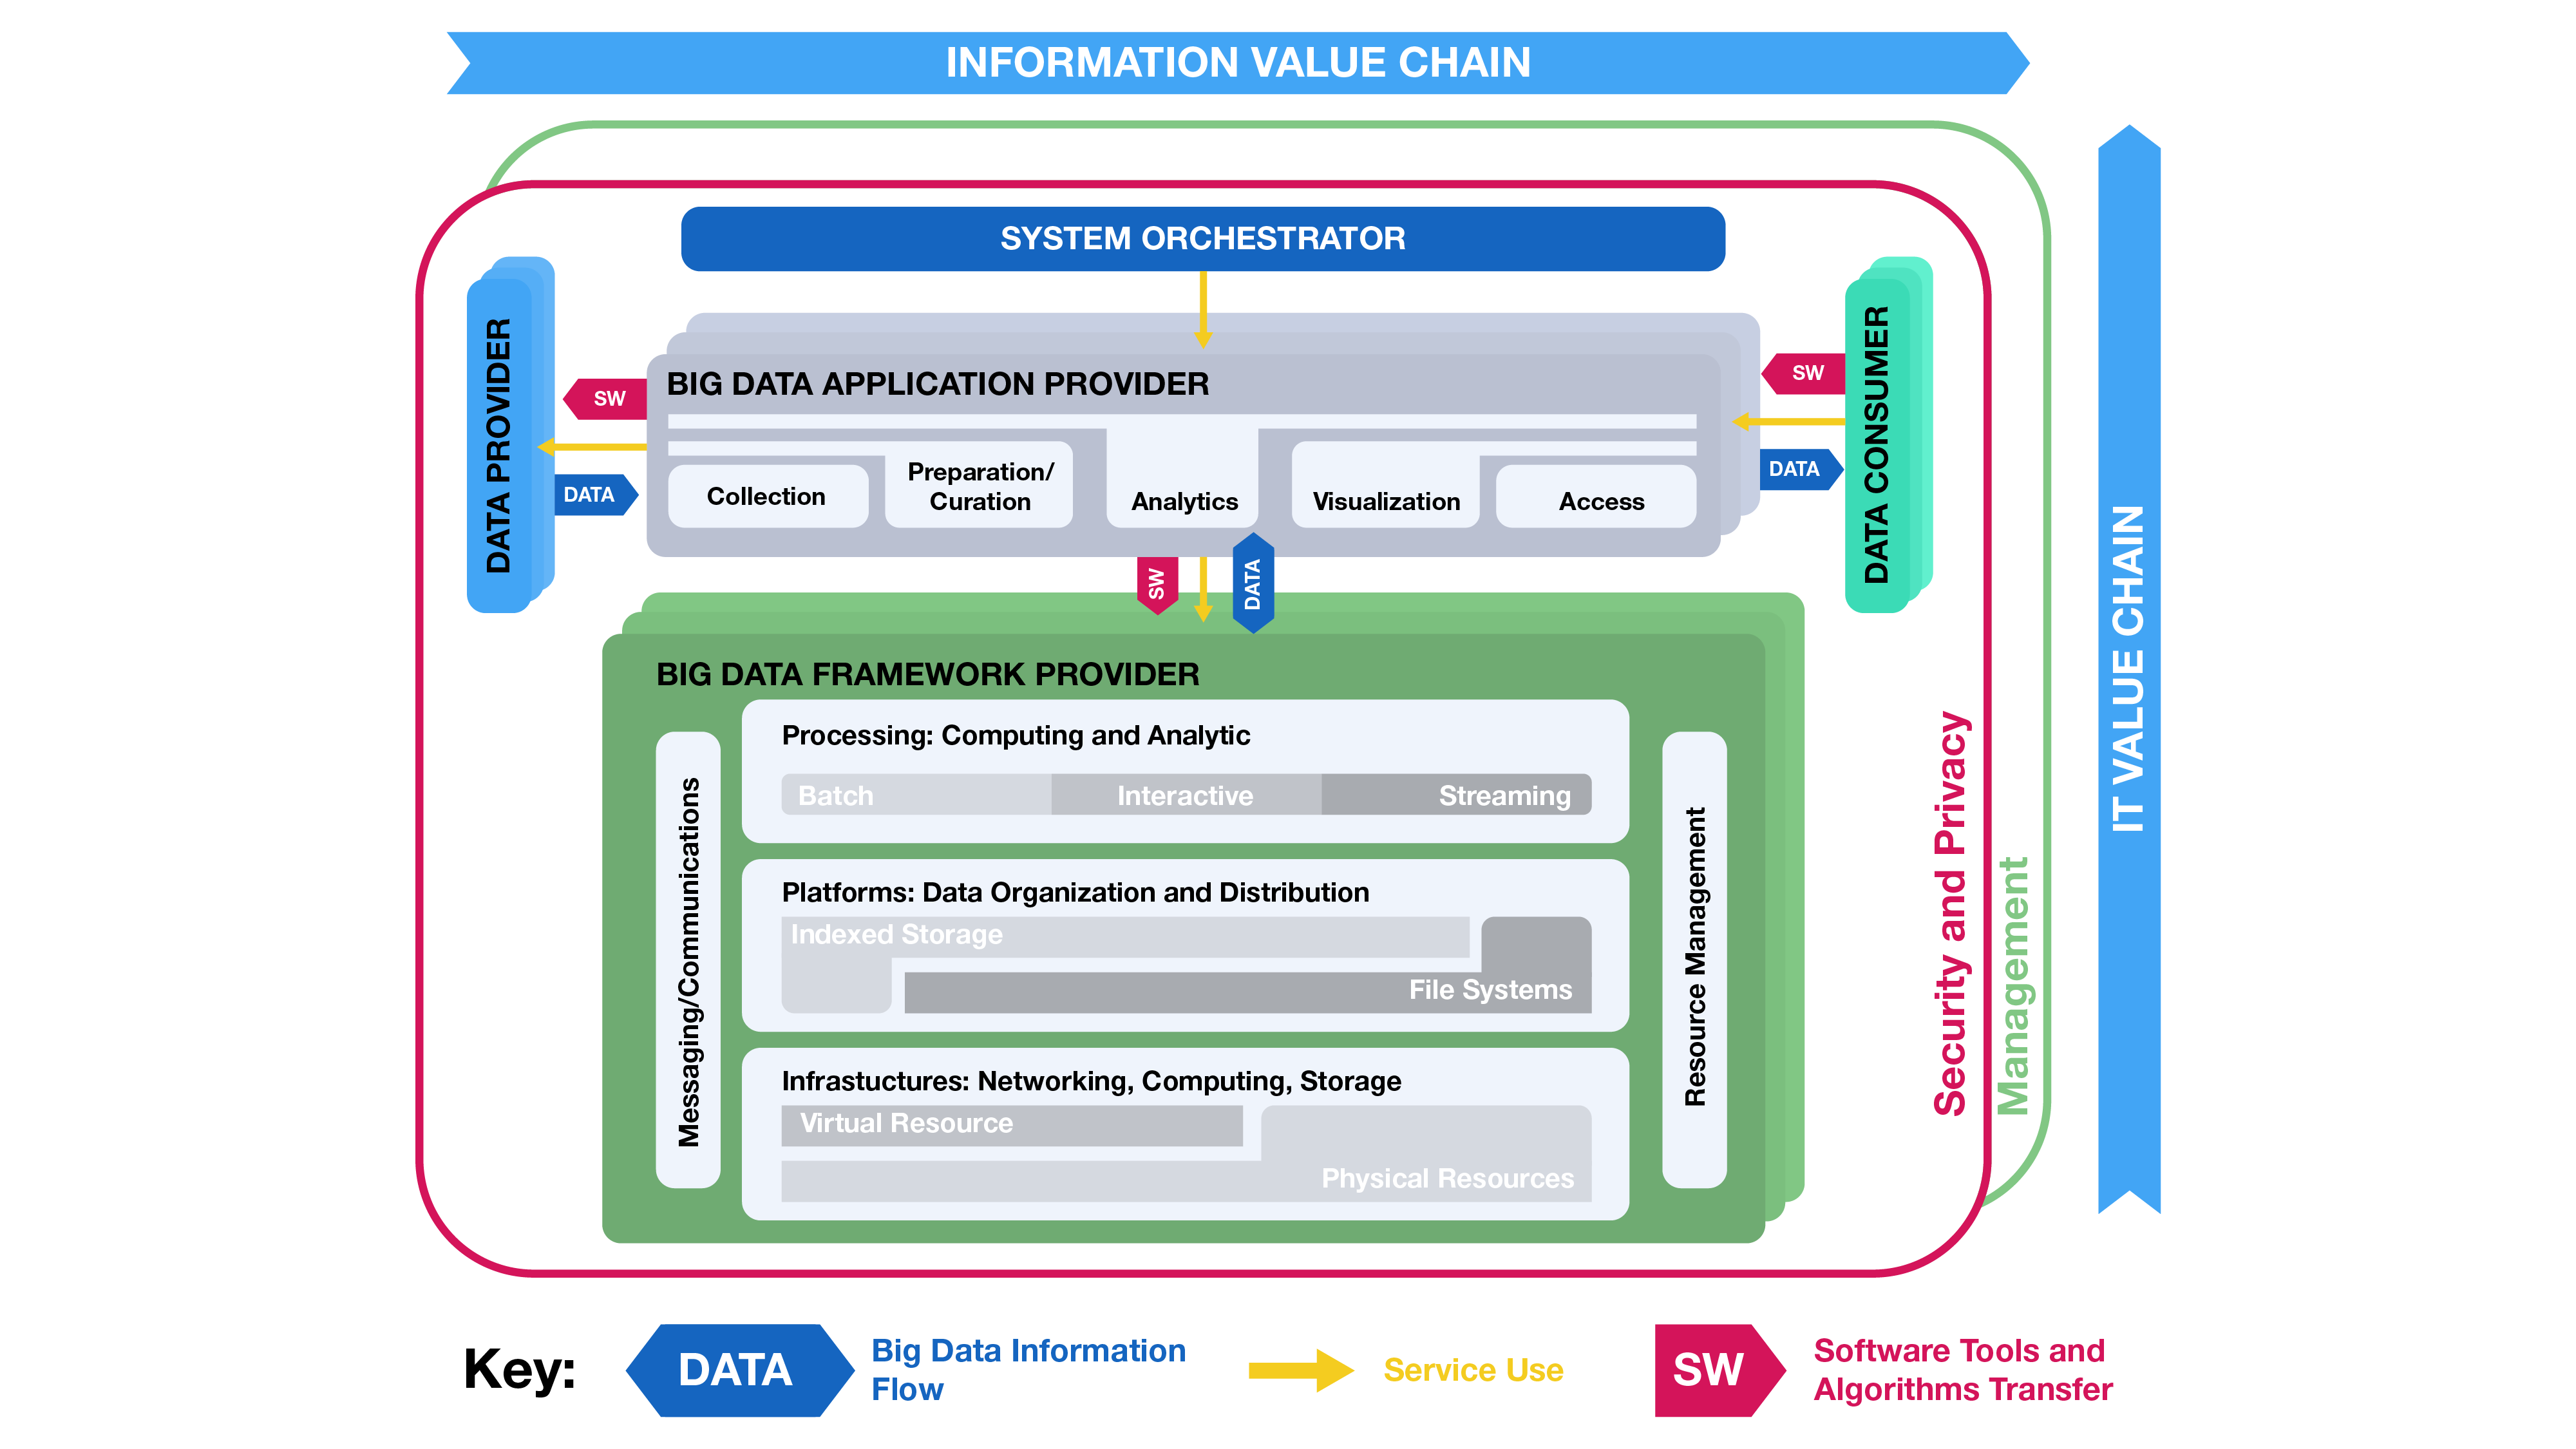
\includegraphics[width=18cm,height=8cm]{imgs/NBDRA_model}
	\caption{NBDRA Conceptual Model}
	\label{fig:NBDRA}
\end{figure*}
I 5 ruoli principali sui 2 assi dei Big Data sono:
\subsubsection{System Orchestrator}
Il system orchestrator coinvolge spesso anche Information Value chain, poiché si preoccupa di implementare e monitorare i processi business a livelli enterprise e le varie politiche sui dati: Redere i dati accessibili per un tempo limitato oppure fornire i dati a velocità diversa(passando il dato in memoria al disco).
Può assegnare/fornire componenti framework fisici o virtuale al sistema, questa assegnazione può essere molto spesso elastica ed indipendente.
Può fornire supporto GUI e collegare i varie applicazioni a un livello alto, e attraverso il management fabbric monitorare i carichi e il sistema per garantire/specificare la qualità del servizio necessaria per i vari carichi.
E' molto spesso centralizzato.
Es. Ambari/Cloudera

\subsubsection{Data Provider}
Può essere sia un software (ad es. in una pipeline più grande) che una persona. Se è una persona metterà i suoi dati e userà gli strumenti di collection e curation/preparation per caricare i dati sul sistemi e migliorarne la qualità, Se un software metterà is suoi dati a disposizione attraverso delle interfacce come Apache Scoop. 
Il data provider può essere interno o esterno alla piattaforma, deve fornire i diritti di accesso ai dati, ed è obbligato a seguire le policy di privacy e security fabbric. 
I dati possono essere inseriti in pull o push.
es. Flume per caricare i dati da MySQL a HDFS.

\subsubsection{Data Consumer}
Riceve i output dei sistemi BigData, può anche lui fare pull e push dei dati, può usare le informazioni per data reporting, retrival/search e visualization. Ci deve essere l'autenticazione ed autorizzazione da parte della privacy and security fabbric per la comunicazione tra l'architettura e il Data Consumer.

\subsubsection{Big Data Application Provider}
Corrisponde alle attività tipiche di un Data Scientist, che esistono anche nei sistema tradizionali ma hanno delle trasformazioni nella implementazioni con i Big Data. Queste attività sono:
\begin{myitemize}
	\item Collection: Si occupa di gestire l'interfaccia fornita dal Data Provider, salva/gestisce questi dati in una certa zona affinché questi non vengano persititi, inoltre implementa funzionalità di estrazione dati dal data provider;
	\item Preparation: Effettua Data Validation, rimozione outlier, standardizzazione, formattazione e arricchimento. 
	Cerca di promuovere dati di alta qualità;
	\item Analytics: Estrazione conoscenza dai dati, sfruttando il software sottostante del Big Data Framework Provider;
	\item Visualization: Presentazione dati in maniera visuale;
	\item Access: E' l'opposto della collection, si preoccupa di esporre i dati verso l'esterno. 
\end{myitemize}

\subsubsection{Big Data Framework Provider}
Fornisce le infrastrutture per supportare i Big Data Application Provider. Si occupa in particolare di:
\begin{myitemize}
	\item Processing dei dati - ha una dualità: da una parte è un framework che mette a disposizione delle interfacce per la programmazione per fare certe cose (es. MapReduce) e dall'altra parte definisce come l'implementazione viene effettuata. I framework possono variare tra un proccessamento batch e in streaming.
	\item Platforms per l'organizzazione e immagazzinamento dei dati - può contenere i meta-dati insieme alle descrizione semantiche dei dati. 
	Può sia essere relazionale distribuito che non relazionale.
	\item Infrastructures per l'esecuzione fisica del nostro software, è l'insieme delle risorse computazionali fisiche o virtuali sulle quali il nostro sistema Big Data gira, può essere costituito da server di grandi o piccole dimensione. 
	Queste componenti forniscono:
	\begin{myitemize}
		\item Networking - Possono essere definiti attraverso software e possono essere reti fisiche che può essere a sua volta partizionato in reti virtuali. 
		Possono essere reti puramente virtualizzate cioè tutto quanto (firewall, router, load balancing) è realizzato in maniera virtuale (es. VM dentro la nostra macchine);
		\item Computing - Hardware, Software, OS, memoria per il computing;
		\item Storage - dischi per storare (in locale), RAID, in rete ecc.;
		\item e altri servizi come il Raffrendamento, l'apparto elettrico e la sicurezza
	\end{myitemize}
	Può essere deployato su ambienti fisici che virtualizzati (nativi, hostati o contenerizzati).
\end{myitemize}
Inoltre ha 2 ruoli diffusi nelle 3 componenti sopraindicate:
\begin{myitemize}
	\item Comunicazione e messaggistica tra le componenti;
	\item Gestione delle risorse per l'integrazione delle componenti.
\end{myitemize}

\subsection{I 2 ruoli diffusi per Big Data}
Questi 2 ruoli prendono il nome di Fabric, il termine Fabric(tessuto) viene usato perché questi due ruoli sono cross-cutting, cioè sono presenti un pò ovunque nell'architettura.

\subsubsection{Management fabbric}
Le due attività principali associate sono:
\begin{myitemize}
	\item Gestione del sistema per provvedere le risorse, gestione dei software e pacchetti e infine la gestione delle configurazioni e performance delle varie pipeline;
	\item Ciclo di vita dei Big Data, BDLM (Big Data Life Cycle Management), contiene l'enforcing delle Policy (es. encoding/decoding), gestione dei meta data (data governance), accessibilità dei dati, data recovery e la loro preservazione.
\end{myitemize}


\subsubsection{Security and Privacy Fabric}
Si occupa delle tre caratteristiche tipiche delle security: 
\begin{myitemize}
	\item Autenticazione: Indica tutte le attività che validano l'utente;
	\item Autorizzazione: Una volta autenticato l'utente verifica i suoi permessi, es. alcuni dati potrebbero non essere accessibili a certi utenti;
	\item Auditing: riguarda la registrazione degli eventi che accadono nel sistema, può far partire un allarme in caso di evento anomalo o a posteriori analizzare la sequenza di eventi (con i file log).
\end{myitemize}

\section{Virtualizzazione}
Per i computer sono stati definiti con le 5 componenti classiche:
\begin{myenumerate}
	\item Input Devices: Tastiera ecc.
	\item Output Devices: Display ecc.
	\item Storage Devices: Volatile(RAM), Permanente(HD, SSD)
	\item Processore:
	\begin{myitemize}
		\item Datapath
		\item Control
	\end{myitemize}
	\item Network
\end{myenumerate}
La virtualizzazione permette l'esecuzione di più sistemi operativi simultaneamente sulla macchina in maniera totalmente isolata. 
Può essere visto come una emulazione di un software o hardware su cui altri software possono eseguirsi, questo ambiente emulato è detto virtual machine.
Il concetto di VM è stato sviluppato negli anni 60 da IBM sui mainframes.
Viene abbandonato con la nascita di PC moderni e ripreso con la crescita recente di cloud. La virtual machine viene ottenuto attraverso un Virtual Machine Monitor (VMM) detto anche ipervisore.\\
L'\textbf{Hypervisor}(Ipervisore) è un software che giace sotto gli OS virtualizzati per offrire le funzionalità di condivisione delle risorse disponibili in modo tale che il programma o OS in esecuzione veda queste risorse come se fosse a lui dedicate. 
Le risorse sono CPU, memoria, storage e la rete.\\
Vi sono diversi benefici della virtualizzazione:
\begin{myitemize}
	\item Visione unificata delle risorse es. vedo tanti dischi come un unico disco;
	\item Consolidazione delle risorse virtualizzate, in modo da avere utilizzo ottimale delle risorse;
	\item Facilità nell'implementazione della ridondanza per copiare gli ambienti virtualizzati;
	\item Facilità la migrazioni di sistema su un altro, inoltre se non cambio ipervisore la macchina(virtuale) funzionerà identicamente a prima;
	\item Gestione centralizzata del hardware e software.
\end{myitemize}
Altri benefici/proprietà della virtualizzazione sono:\\
\textbf{Workload Isolation:} attraverso la virtualizzazione è possibile isolare completamente i programmi, che ha miglioramenti anche nella sicurezza, inoltre aumenta affidabilità poiché il fallimento di un programma non comporta fallimento dei programmi poiché sono isolati, inoltre si risolvono anche i problemi riguardanti i conflitti di librerie in questo modo. Infine si ottiene un controllo sulle performance poiché l'esecuzione di una VM non affligge il performance dell'altra;\\
\textbf{Workload Migration:} ciò aiuta in:
\begin{myitemize}
	\item Mantenimento di Hardware;
	\item Load Balancing;
	\item Fault Tolerance;
	\item Disaster Recovery.
\end{myitemize}
Poiché possiamo spostare tutto l'ambiente virtualizzato su una nuova macchina in maniera abbastanza trasparente, per fare ciò la macchina dovrebbe essere sospesa, totalmente serializzata per essere inviata nella rete, migrata su una nuova macchina e fatta ripartire immediatamente o solo salvata senza esecuzione.\\
\textbf{Consolidazione:} Sfruttando il Workload Migration è possibile consolidare macchine separate su un unica piattaforma riducendo i costi (usata molto spesso nei Datacenter in orari non di picchi).\\
\begin{figure}[h]
	\centering
	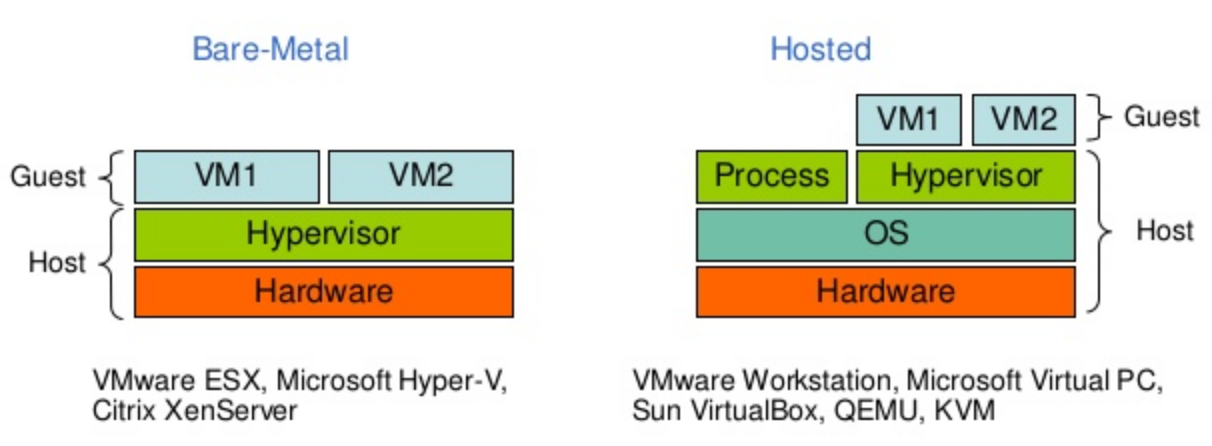
\includegraphics[width=\linewidth]{imgs/hypervisor_type.png}
	\caption{I tipi di Hypervisor}
	\label{fig:hypervisor_type}
\end{figure}
I diversi tipi di HyperVisor sono (Fig \ref{fig:hypervisor_type}):
\begin{myitemize}
	\item \textbf{Hosted}: in questo caso l'ipervisore è un processo che gira al di sopra del sistema operativo e permette l'esecuzione di più macchine Guest.
	In questo caso quindi bisogna installare prima un OS su cui verrà installata VMM (ipervisore) e a questo punto l'host potrà eseguire le applicazioni all'interno della sua finestra.
	Il vantaggio qua è la facilità di installazione e configurazione, inoltre la HostOS e GuestOS rimangono non modificati e non dipendono dal particolare hardware, ma gli svantaggi sono la degradazione delle performance e la mancanza di supporto real time OS poiché vi sono varie entità/software in mezzo;
	\item \textbf{Bare-Metal}: in questo caso l'ipervisore funziona direttamente al di sopra del Hardware.
	In questo caso l'ipervisore è un OS molto leggero e comunica direttamente con hardware al posto di dipendere su un altro OS. 
	I vantaggi sono miglioramento in I/O e supporto real time, mentre gli svantaggi sono la difficoltà di installazione e configurazione e la dipendenza dal tipo di hardware specifico.
\end{myitemize}
Ci sono principalmente 2 tecniche di virtualizzazione: \textbf{Software Virtualization} (di cui abbiamo parlato fino ad adesso) e \textbf{Hardware Assisted Virtualization}.\\
Nella \textbf{Virtualizzazione Totale} VMM si preoccupa di emulare in maniera completa tutto l'hardware, quindi avremo un processore, memoria, disco e network virtuale.
In questo caso OS ospite non è consapevole dell'esistenza dell'ambiente virtuale e ogni macchina è del tutto indipendente.
A livello CPU, avviene la traduzione binaria: Questo avviene in diversi anelli di sicurezza, in particolare gli anelli sono 4, dove l'anello 0 è quello più privilegiato e permette l'esecuzione del codice direttamente sul hardware e qua viene eseguito il kernel dell'OS.
Le applicazione dell'utente vengono eseguite sull'ultimo anello (anello 3).\\
L'ipervisore gira sull'anello 0 mentre le GuestOS gira sull'anello 1, quindi hanno più permessi delle normali applicazioni. 
VMM ha accesso sul anello 0 per avere accesso diretto sulla CPU piuttosto che virtualizzarla. \\
La \textbf{Para-Virtualizzazione} ha un approccio diverso rispetto alla virtualizzazione totale (è una via di mezzo tra total virtualization e bare-metal), in questo caso il Guest sono consapevoli della VMM e usa chiamate speciali in alcuni casi per essere eseguite direttamente sul hardware e ciò comporta un miglioramento nella performance ma ciò lo rende meno flessibile.\\
La \textbf{OS-level Virtualization (Containerization)} non usa la VMM, la virtualizzazione è fornita direttamente dal HostOS che esegue tutte le funzioni di un ipervisore totalmente virtualizzato, quindi ha una partizione puramente virtuale delle risorse, e ciò comporta un'assegnazione flessibile delle risorse alle varie applicazioni. Es. Docker.\\
Ci sono 3 modelli di servizio:
\begin{myenumerate}
	\item \textbf{Server Virtualization}: supponiamo di avere diversi server su macchine diverse, in caso di un problema (crash di un nodo) o vi è un bisogno di upgrade, in caso di macchine fisiche dovrò prendere lo stesso modello o lo stesso vendore, la soluzione è quella di sfruttare una medesima macchina con un virtualizzatore e mettere i diversi server insieme.
	In questo modo ho una consolidazione, risorse condivise, una gestione centralizzata, facilità di migrazione, maggiore ROI e meno spazio occupato.
	La Disaster Ricovery e scalabilità viene facilitata, diversi modelli (hardware) a scelta (basta che sia uguale l'ipervisore) e ho maggiore disponibilità.
	\item \textbf{Desktop Virtualization}: è la tecnologia che separa l'ambiente desktop e le applicazione software dal cliente fisico che lo usa. 
	Il nostro desktop diventa un thin client che usa PC privo della memoria RAM e potenza calcolo necessaria per far funzionare una macchina reale, la macchina gira su un pool di VM su un server su un data center.\\
	I benefici sono molteplici: Upgrade di software e OS facilitato, alta disponibilità, fault tolerance, accessibile da LAN, WAN, Internet, inoltre vi è la possibilità di far eseguire una piccola parte della computazione dal dispositivo locale.
	\item \textbf{Application Virtualization}: Molto simile alla Desktop Virtualization, solo che al posto di tutto il desktop, sono le applicazione ad essere in virtualizzate, quindi un applicazione che gira sul desktop, fa la computazione sul cloud, una piccola parte della computazione può essere effettuata anche in locale.
	I vantaggi sono molto simili a quelli del Desktop Virtualization, un vantaggio aggiuntivo può essere che pago solo quello che uso, riducendo i costi delle licenze.
\end{myenumerate}
%\section{Lezione 3 - 09/10}

\section{Cloud}
Definizione ``vera'' del cloud da ricordare: è un tipo di servizio distribuito di sistemi interconnessi e computer virtualizzati dinamicamente provvisionati e presentati come un unica risorsa computazionale basato su service-level agreement.
\\
Sostanzialmente il cloud è la possibilità di avere accesso alle risorse computazionale attraverso la rete on-demand ed è composto da 5 punti chiave, 3 modelli di servizio e 4 modelli di deployement.

\subsection{The 5 Properties of cloud}
Le 5 proprietà aggirano attorno ad una idea centrale del cloud: Utility Computing, SOA (Service Oriented Architecture) + SLA(Service Level Agrement).\\
\textbf{Utility Computing} nel senso che il service provider fornisce le risorse computazionali e le infrastrutture che servono al cliente e li fa pagare in base all'utilizzo piuttosto che con un costo fisso, come i servizi on-demand, per massimizzare l'uso efficiente, minimizzando i costi nella maniera meno trasparente possibile(senza mostrare al cliente tutto ciò che si fa).\\
\textbf{SOA (Service Oriented Architecture)}: è un insieme di servizio che comunicano tra di loro poiché non basta di solito un solo servizio per implementare un servizio web completo per utente.\\
\textbf{SLA (Service Level Agreement)}: è un contratto tra il service provider e il cliente che specifica il livello di servizio che il service provider deve fornire in termini di QoS.
Il \textbf{QoS}(Quality of Service) è un set di tecnologie per gestire il traffico della rete in modo da migliorare la user experience, ormai è associato a un significato più generico riguardante le valutazioni di tecnologie non funzionali, cioè non mi interessa solo la funzionalità (il risultato della mia richiesta) ma anche la sua efficienza.\\
Le metriche più comuni delle SLA sono up-time e down-time, Response time. Se le metriche garantite non vengono rispettato vi sono delle penalità sui service provider.\\
La tecnologia grazie al quale cloud funziona sono:
\begin{myitemize}
	\item Hardware Virtualization;
	\item Computing distribuito e parallelo;
	\item Service-oriented Computing;
	\item Autonomic Computing (reazione a cambiamenti del sistema).
\end{myitemize}

Le 5 \textbf{proprietà/caratteristiche} che identificano il cloud sono:
\begin{enumerate}[noitemsep, topsep=0ex, leftmargin=*]
	\item \textbf{Scalabilità, Elasticità}:
	\begin{itemize}[noitemsep, topsep=0ex, leftmargin=*]
		\item Scalabilità è una proprietà del sistema di crescere in maniera graduale col crescere di richieste, può essere orizzontale (Scale In \& Scale Out) o verticale (Scale Up \& Scale Down).
		\item Elasticità è l'abilità di adattarsi automaticamente per inizializzare la scalabilità.
	\end{itemize}
	Ciò si può ottenere attraverso provisioning dinamico, che fa riferimento è un ambiente complesso che permette la allocazione e de-allocazione on-demand delle istanze/risorse attraverso applicazione o un console amministrativo. 
	Di solito vengono messe delle regole per automatizzare il provisioning, ottenendo così un abbassamento dei costi e performance migliorata.
	
	\item \textbf{Disponibilità, Affidabilità}:
	\begin{itemize}[noitemsep, topsep=0ex, leftmargin=*]
		\item Availibility è il rapporto tra il up-time e tempo totale di esecuzione;
		\item Affidabilità è la capacità di funzionare in situazioni particolari (rottura di un nodo, attacco di hacker) per un certo tempo.
	\end{itemize}
	Questi punti possono essere ottenuti attraverso sistemi di:
	\begin{itemize}[noitemsep, topsep=0ex, leftmargin=*]
		\item Fault Tolerance è la capacità del sistema di continuare ad funzionare anche dopo un fallimento di uno dei suoi componenti, spesso il servizio viene degradato proporzionalmente alla gravità del fallimento ma il servizio continua ad funzionare.\\
		Le caratteristiche principali sono che non ha un singolo punto di fallimento, la componente fallita viene individuata ed isolata per prevenire la propagazione del fallimento;
		\item Resilience è l'abilità di offrire e mantenere un livello di servizio accettabile anche dopo un fallimento, essenzialmente ritornare allo stato di funzionamento dopo un caso di fallimento del sistema (ad es. viene a mancare l'elettricità).
		Quindi i sistemi devono avere le policy e procedure per il recupero, ad es. Backup (dei dati off-site oppure di tutto il sistema) oppure preparazione contro fault come un una corrente non-interrompibile (UPS) oppure sbalzi di corrente/tensione.
		\item Sicurezza, che riguarda l'impiego di politiche e tecnologie e sistemi di controllo per protegge applicazioni e infrastrutture da accessi malevoli, quindi abbiamo il suo impiego in:
		\begin{itemize}[noitemsep, topsep=0ex, leftmargin=*]
			\item la protezione i dati, mantenendo l'accesso ai dati riservato solo in base ai privilegi;
			\item Gestione dell'identità per garantire l'accesso alle risorse in base ai loro privilegi (protezione dei dati);
			\item Sicurezza dell'applicazione riguarda la possibilità di blindare le nostre applicazioni per accessi malintenzionati;
			\item Privacy per oscurare i dati in base alle leggi privacy e gestiti solo da utenti competenti.
		\end{itemize}
	\end{itemize}

	\item \textbf{Gestibilità, Interoperabilità}:
	La Gestbilità riguarda la gestione di questi sistemi attraverso un singolo punto di accesso mentre la interoperabilità è una proprietà di un prodotto o sistema per lavorare con altri prodotti/sistemi.
	Lo si ottiene attraverso \textbf{System control automation} e \textbf{System State Monitoring} che è un processo che monitora lo stati dei hardware, metriche dei performance, i log dei sistemi, il pattern dei accessi alla rete ecc.
	E' anche collegato al sistema di Billing, poiché gli utenti pagano ciò che usano e il cloud provider deve registrare le risorse/servizio usate da ciascun utente.\\
	\item \textbf{Accessibilità, Portabilità}
	
	\item \textbf{Ottimizzazione, Performance}
	Il \textbf{Load Balancing} è una tecnica per la distribuzione del workload su un sistema di più computer, CPU, HD ecc. per ottenere l'utilizzo ottimale, migliorando così: l'utilizzo del sistema, la performance e l'efficienza energetica riducendo overload.\\
	Il \textbf{Job Scheduler} è un applicazione che ha il compito di eseguire i processi in background (chiamati anche processi batch).
	Nel cloud i task intensivi computazionalmente o task che crescono dinamicamente vanno pianificati con Job Scheduler.
\end{enumerate}
Da un punto di vista dell'utente, lui non vuole sapere come e cosa viene fatto né chi gestisce il servizio, ma vuole solo un servizio funzionale.

\subsection{The 3 Service Model of cloud}
Iniziamo con i tre modelli del servizio del cloud sono:
\begin{enumerate}[wide, topsep=0ex, noitemsep]
	\item \textbf{IaaS (Infrastructure as a Service)}: es. le macchine virtuali, in questo caso il provider/vendor gestisce la virtualizzazione, il cliente ottiene le risorse virtuali, di solito da un catalogo che contiene le specifiche hardware (virtualizzato) pre-selezionate dal provider. Nella maggior parte dei casi gli OS sono anche prefissate per questioni di prestazioni/stabilità e compatibilità con hypervisor da loro usato. Gestito di solito da un system administrator.
	\item \textbf{PaaS (Platform as a Service)}: ci viene fornito una scatoletta dove scrivere ed eseguire/testare le applicazioni, il provider sarà il garante del fatto che il sistema sia abbastanza responsive e abbia un runtime sufficiente. E' meno flessibile rispetto allo IaaS ma allo stesso momento lo sviluppatore perde meno tempo nella configurazione delle macchine. Gestito di solito da sviluppatori.
	\item \textbf{SaaS (Software as a Service)}: es. GMail quindi utente non può fare niente tranne usare il software. Usato da utenti o business analyst.
\end{enumerate}

In realtà il cloud vero è un po' più offuscato di quanto detto sopra, spesso non è facile collocare il modello di cloud di un'azienda esattamente in uno dei 3 modelli.\\
Un aspetto molto importante da considerare è quello economico, cioè grazie al modello pay-as-you-go cloud il costo capitale (CAPEX) si trasforma in costo operazionale (OPEX), inoltre il rischio di errore nella scegliere le macchine sparisce, se ho bisogno di più potenza richiedo una macchina più forte e se ho bisogno di meno potenza abbasso la potenza e risparmio.
Allo stesso momento i cloud service provider hanno diversi benefici: profitto sfruttando l'economia di scala (comprare un servo costa X, ma comprare N server non costa N*X), possono capitalizzare sui loro investimenti (amazon che vende la potenza residua) o possono sfruttarlo per promuovere un loro prodotto (es. per far usare .NET ai sviluppatori).

\subsubsection{IaaS}
IaaS fornisce automaticamente il processing, storage, network e altre risorse fondamentale per il computing, e l'utente può installare i software che sono per lui necessari.\\
Lo IaaS supporta queste 3 caratteristiche del cloud:
\begin{myitemize}
	\item Gestibilità e Interoperabilità: Attraverso un interfaccia può gestire tutte le VM che vuole, le può pagare come vuole;
	\item Disponibilità ed Affidabilità: gestita dal cloud provider attraverso le zone di disponibilità;
	\item Scalabilità ed elasticità: Proprietà del sistema ma deve essere implementato dall'utente.
\end{myitemize}
L'architettura è composta dall'hardware seguita da un layer di virtualizzazione e l'utente ha accesso a due interfacce:
\begin{myitemize}
	\item Interfaccia per gestione delle risorse, queste risorse sono:
	\begin{myitemize}
		\item VM: creazione, cancellazione, gestione, sospensione delle VM 
		\item Virtual Storage: Allocare spazio, ridurre/aumentare del DB, scegliere servizi con velocità di lettura/scrittura diversi (per prezzo);
		\item Virtual Network: gestione delle IP associate alle VM, registrazioni al dominio delle IP, scegliere la larghezza di banda.
	\end{myitemize}
	\item Interfaccia del il monitoring del sistema: viene messa a disposizione da VIM: L'orchestrazione delle macchine/risorse, in maniera rapida e dinamica, su un server viene gestita dalla Virtual Infrastructure Mangaser(VIM), diverse metriche vengono usate per il monitoraggio es:
	\begin{myitemize}
		\item VM: CPU usage, memory usage;
		\item Virtual Storage: utilizzo del disco, livello di duplicazione dei dati e velocità di accesso al disco;
		\item Virtual Network: L'uso della banda, lo stato di connettività e il bilanciamento sulla rete.
	\end{myitemize}
\end{myitemize}


\subsubsection{PaaS}
PaaS mette a disposizione dell'utente i linguaggi di programmazione e i tools (come IDE) supportati dal provider, quindi il controllo sul deployement dell'applicazione è nelle mani del consumer ma le infrastrutture sottostanti sono gestite dal cloud provider.
\\
Alla base vi è una archittettura come quella di IaaS, vengono aggiunti i Runtime Environment e sopra questi ci sono i Programming IDE e le API/tools supportati dall'ambiente, spesso hanno in comune le funzioni come: computation e lo storage.\\
Il Runtime Environment si riferisce a una collezione di software, implementati con una collezione di librerie, le proprietà fornite dal Runtime Environment sono:
\begin{myitemize}
	\item Gestibilità ed Interoperabilità
	\item Performance ed Ottimizzazione
	\item Disponibilità ed Affidabilità
	\item Scalabilità ed Elasticità
\end{myitemize}
L'interfaccia messa a disposizione per il controllo del sistema mette a disposizione un set di azioni in base a:
\begin{itemize}
	\item Policy based control: le azioni seguono delle regole per prendere delle decisioni quindi azioni seguite con if $<>$ then $<>$
	\item Controllo del workflow: descrizione del flusso di installazione e configurazione delle risorse oppure dei daemon.
\end{itemize}

\subsubsection{SaaS}
SaaS: vengono fornite al cliente applicazione del provider in cloud, l'utente non può gestire o sviluppare l'applicazione o gestire l'architetture nel cloud ma può interagire con esso attraverso interfacce ad es. portali/applicazioni web, che con introduzione del Web 2.0 ha potenziato l'iterabilità con l'applicazione in cloud, es: Facebook(Messenger), Office, Skype, DropBox, sistema CRM, sistema medico nazionale, sistema di trasporto pubblico.\\
Il punto fondamentale di questo tipo di cloud è l'Accessibilità e la portabilità.\\
Oss: La differenza tra il portale web e una pagina web è che il portale permette l'integrazione di diverse pagine attraverso dei login.

\subsection{The 4 Cloud Deployement Models}
I 4 modelli primari che differenziano un cloud, basati sulle possibilità di accesso, la dimensione e la proprietà dei servizi, sono:
\begin{myitemize}
	\item \textbf{Public Cloud} (o multi-tenant o external cloud): 
	L'infrastruttura viene messa a disposizione del pubblico generale o almeno alle organizzazioni grandi attraverso pagamento per il suo uso, le caratteristiche sono:
	\begin{myitemize}
		\item Infrastruttura omogenea per garantire le medesime prestazioni a due utenti che pur trovandosi in posti diversi usano lo stesso servizio;
		\item Policy comuni;
		\item Risorse condivise;
		\item Infrastrutture viene affittata;
		\item Economia di Scala.
	\end{myitemize} 
	
	\item \textbf{Private Cloud:} (o on-premise cloud o internal cloud)
	Viene operato da un'unica organizzazione e può essere gestita dalla stessa o un'altra organizzazione, cioè la categoria di utenti è limitata. A differenza del public cloud le caratteristiche sono:
	\begin{myitemize}
		\item Infrastruttura eterogenea per via del costo e dal fatto che una azienda privata non butta via un hardware solo per averli omogeneità;
		\item Policy customizzate ad-hoc per gli utenti;
		\item Risorse dedicate;
		\item Infrastrutture gestita da house;
		\item End-to-end control sui processi.
	\end{myitemize}
	
	\item \textbf{Community Cloud:} è una struttura gestita da diverse entità, in pratica più entità mettono insieme i loro cloud privati per generare un super cloud, ad esempio alcune università americane possono unire i loro cloud per qualche ricerca specifica ecc.
	
	\item \textbf{Hybrid Cloud:} è la comoposizioni di più tipi di cloud, ad esempio un azienda privata crea il suo cloud privato per la gestione di informazioni sensibili e usa il cloud pubblico per il resto, oppure lo usa per la scalabilità in caso di traffico aumentato.
\end{myitemize}

\section{Amazon ECOSYSTEM-IaaS}
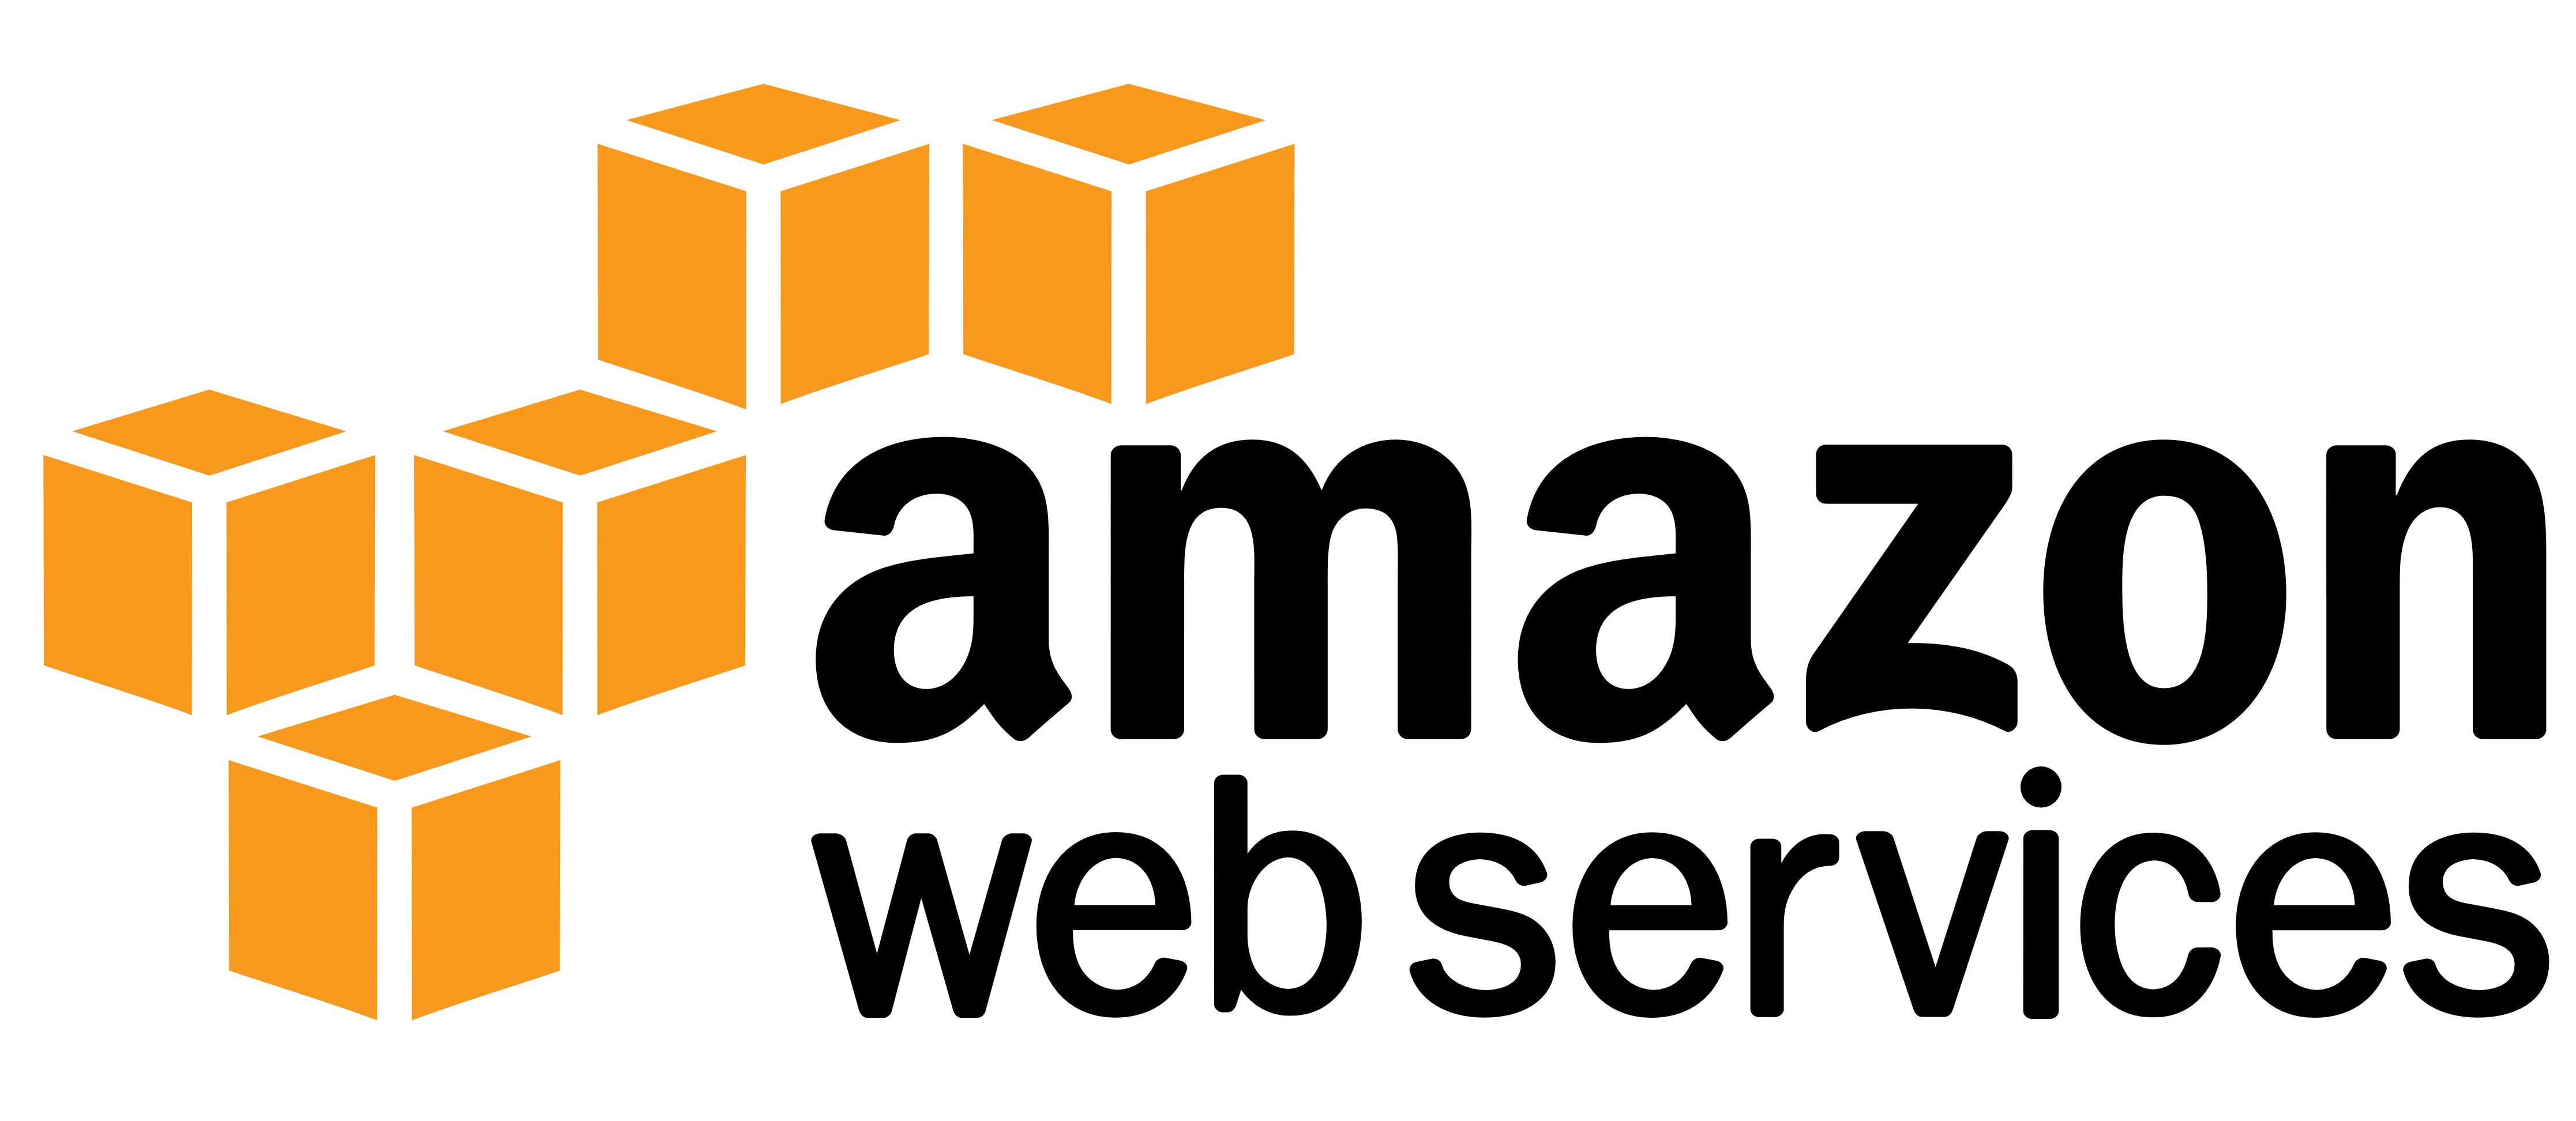
\includegraphics[width=1.5cm,height=0.5cm]{imgs/AWSLogo.png} sono creati per lavorare indipendentemente ma possono interagire tra di loro, condividendo tra di loro le stesse convenzioni di nomi e autenticazione e minimizzando le connessioni interne.
\\
Amazon mette a disposizione il concetto di regione e di zona di disponibilità:
\begin{itemize}[noitemsep, topsep=0ex, wide]
	\item Ciascuna \textbf{Availibility Zone} è un data center indipendente con la propria griglia di potenza e connessione della rete, le zone all'interno di una regione sono collegate tra di loro attraverso connessione a latenza bassa. 
	Il nome deriva dal fatto che sono zone ad alta disponibilità, quindi se una zona fallisce il suo effetto non viene notato dalle altre zone creando così una stabilità ed alta fault tolerance.
	\item \textbf{Regione} è un cluster di Availibility Zone localizzati in una area geografica. 
	Quando si crea una istanza Amazon ci dà la possibilità di scegliere una availability zone (o di default lo si lascia far scegliere ad Amazon) e all'interno della stesso regione è possibile distribuire la propria istanza su più availability zone, quindi se una zona fallisce l'altra (molto probabilmente) continua a funzionare.
	Amazon non fa pagare i trasferimenti di dati all'interno della stessa regione, ma tra regioni le comunicazioni vengono fatte pagare.
\end{itemize}
Esiste AWS GovCloud che è una regione AWS isolata e permette di gestire dati estremamente sensibili e può essere acceduta solo da cittadini Americani verificate dal governo Americano e sul suolo Americano.\\
Uno dei servizi principali di AWS è \textbf{Simple Storage Service (S3)}, un storage object che è un sistema di archiviazione piatto cioè non è possibile creare cartelle al suo interno, i dati vengono salvati in formato binario e vengono distribuite automaticamente. 
L'accesso può essere effettuato da chiamate web (REST, Soap, BitTorrent) o query SQL e gli oggetti possono anche essere molto grandi (fino a 5TB ciascuno).\\
S3 sta alla base di tutta l'infrastruttura che sta alla base di Amazon e-commerce.
Oltre a S3 Amazon fornisce anche un \textbf{EBS (Elastic Block Store)}, questo disco può essere formattato, montato e usato come hard disk locale, è un volume che persiste indipendentemente dal resto.
Mentre le VM possono morire, i volumi rimangono sempre, e la garanzia di durabilità viene fornita da Amazon.\\
EBS è categorizzato in SSD e HDD, a seconda del tipo di macchine/dischi si paga in maniera diversa.\\
I \textbf{Security Group} definiscono l'insieme delle connessioni possibili per una certa istanza, e questi insiemi possono essere protocolli, porte, range delle IP.

\subsection{EC2 - Elastic Cloud Computing}
\textbf{EC2(Elastic Cloud Computing)} è uno dei servizi offerti per la creazione/gestione delle macchine virtuali on-demand. EC2 si basa sul concetto di data center programmabile, la possibilità di creare una propria infrastrutture (macchine in più availability zone o regioni) tramite linguaggi di programmazione.
I concetti chiave che constituiscono EC2:
\begin{myitemize}
	\item \textbf{Amazon Machine Image} (AMI): è un file contenente una descrizione di una VM, cioè eventuali software e le configurazioni, possono essere pre-built, create, modificate e vendute. Ciascun AMI ha un ID unico;
	\item \textbf{Istanza}: rappresenta una copia di AMI in esecuzione, multiple copie di un unica AMI può essere messa in esecuzione;
	\item \textbf{Elastic IP address}: allocazione di un IP statico e collegarle alla propria istanza, ciascuna istanza può avere al più un IP statico.
\end{myitemize}
I core messi a disposizione dal server (di cui non sappiamo praticamente nulla) vengono virtualizzati, dividendo prima in core poi dividendo ulteriormente il core-time. L'unità di misura è Elastic Compute units che corrisponde a Intel Xeon (o AMD Opteron) da 1.0-1.2 GHz del 2007.\\
Le risorse possono essere:
\begin{itemize}[noitemsep,topsep=0ex,wide]
	\item Persistenti: anche in caso di fallimento del hardware Amazon ci garantisce la sua persistenza attraverso ridondanza, recupero automatico e failover automatizzato. Le componenti persistenti sono:
	\begin{myitemize}
		\item Elastic IP Address
		\item EBS
		\item Elastic Load Balancer
		\item Security Groups
		\item AMI slavate in S3 o EBS
	\end{myitemize}
	\item Effimere: l'utente deve garantire la sua ridondanza e mantenimento attraverso atri servizi di EC2, in caso di fallimento i dati salvati vengono in generale persi. Le istanze sono effimere.
\end{itemize}
I modelli del prezzo sono:
\begin{itemize}[noitemsep,topsep=0ex,wide]
	\item \textbf{On demand}: Il pagamento avviene per le capacità (tempo) usate con nessun obbligo a lungo termine.
	\item \textbf{Reservati}: Si fa una sorta di abbonamento con un pagamento di una somma prima e poi le macchine si possono usare per la durata dell'abbonamento a un prezzo scontato, è disponibile in 3 tipi Light, Medium e Heavy e può essere per 1 o 3 anni e può far risparmiare fino al 71\% rispetto a On-Demand. Attenzione non ci riserva delle risorse per la durata dell'abbonamento ma solo il prezzo.\\
	\item \textbf{Spot}: Si fa asta per la potenza computazionale non usata da Amazon EC2, sono quelle che costano di meno, perché non mi viene garantita la durata della macchina nel tempo, nel caso il prezzo offerto è maggiore del costo necessario per eseguire quella macchina Amazon darà la sua macchina, ma siccome il prezzo di elettricità è variabile e se dovesse superare il prezzo offerto Amazon può spegnere tale macchina senza avvisare.
\end{itemize}
Un altro indice di costo è \textbf{Data Transfer}, il trasferimento dei dati dentro o fuori dalla istanza EC2 vengono pagati (in base alla quantità) se non il trasferimento avviene al di fuori della regione. 
Il trasferimento dentro la regione è completamente gratuita.\\

\subsection{AutoScaling}
\begin{figure}[!b]
	\centering
	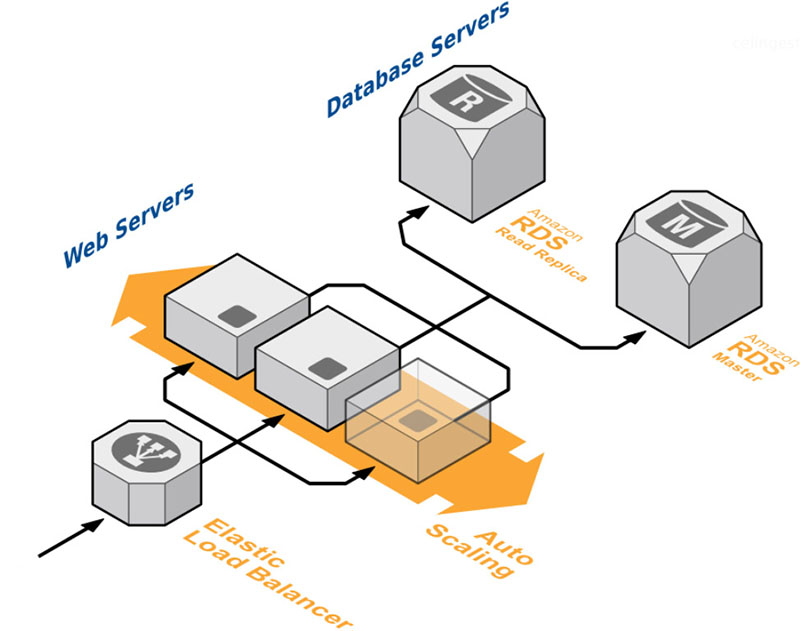
\includegraphics[width=\linewidth]{imgs/load_balancer.jpg}
	\caption{Esempio di Auto Scaling for AWS}
	\label{fig:autoscaleAWS}
\end{figure}
Uno servizio molto importanti di Amazon è \textbf{AutoScaling}(Fig \ref{fig:autoscaleAWS}). Per far funzionare AutoScaling è importante anche il \textbf{Elastic Load Balancer}, grazie al quale l'utente finale vedere solo un collegamento e Elastic Load Balancer pensa a distribuire le richieste alle nostre macchine. 
Le istanze EC2 possono essere categorizzate in auto scaling groups, di solito con un range tra un minimo e un massimo, se una nuova macchina entra in esecuzione oppure viene de-allocata il Load Balancer viene avvertito della modifica in modo che possa funzionare bene.
Gli Auto Scaling group sono istanze EC2 che condividono caratteristiche simili e devono essere fatte per scalare, e aggiunge automaticamente un nuovo nodo in base a policy definite dall'utente, programmazione oppure health checks e workload e la nuova istanza può venire anche da availability zone diverse della stessa regione.\\
Auto Scaling group contiene solo un launch configuration che descrive le istanze che devono far partire (contiene i parametri delle AMI), se si aggiorna il launch configuration questo affliggerà solo le nuove istanze, le vecchie istanze rimangono tali ma esse vengono terminate prima durante un scale in.\\
%\section{Lezione 5 - 16/10}
Attenzione una macchina può essere o spenta o terminata, nel caso viene terminata viene eliminata completamente e AutoScaling group termina una macchina.\\
L'ecosistema di Auto Scaling è composta da:
\begin{myitemize}
	\item Cloud Watch: Per monitorare le istanze EC2, le metriche più usate per il CloudWatch sono:
	\begin{myitemize}
		\item CPU usage
		\item Latenza
		\item Numero di Richieste
		\item Il numero di Host(macchine) in buona salute
		\item Il numero di macchine non in buona salute
	\end{myitemize}
	\item Elastic Load Balancer: Per distribuire il lavoro su un numero qualunque di istanze EC2 ed effettuare controlli periodici sulla salute del nodo (basandosi sul tempo di risposta) e in caso non siano in buona salute il load balancer smette di inviare a lui le richieste.
	\item Auto Scaling: Utilizza i dati collezionati dal CloudWatch per costruire sistemi che possono scalare (dentro o fuori) all'intero del range
\end{myitemize}
Il \textbf{Trigger} è un meccanismo per l'attivazione di una policy, in questo caso di aumentare o diminuire il numero dei nodi. Il trigger può essere attivato da un allarme cloud watch (configurato per guardare una metrica di cloud watch) oppure un auto scaling policy che descrive cosa fare in caso di un allarme. Quando si attiva il trigger lancia un processo chiamato Scaling activity che esegue la auto scaling policy.
Osservazione Auto Scaling supporta ma non necessita Elastic Load Balancer.
In generale almeno due trigger sono necessari, uno per Scale up e uno per Scale down, per mantenere un equilibrio desiderato.
Un allarme è una metrica e verifica se questa metrica supera un limite stabilito per un certo tempo.\\
Un'allarme è un'entità in grado di osservare con continuità una certa metrica e ci indica se tale metrica ha superato un certo valore prefissato per un certo tempo, per creare un allarme è necessario specificare:
\begin{myitemize}
	\item Metrica da osservare
	\item Il threshold della metrica
	\item Il numero di periodo di valutazione
\end{myitemize}
Gli stati in cui l'allarme si può trovare sono:
\begin{myitemize}
	\item Ok, tutto bene! Metrica è sotto il threshold.
	\item Alarm: Metrica è sopra il threshold, è necessaria un azione.
	\item Dati Insufficiente, metrica non disponibile o non ci sono abbastanza dati.
\end{myitemize}
Se l'allarme cambia lo stato e vi rimane per un determinato periodo di valutazione, un'azione viene invocata in base alla policy.\\
I scenari automatici dell'auto scaling sono:
\begin{myitemize}
	\item Fleet Management: assicura il performance ottimale della macchina, controllando la salute dell'istanza con Health Check: se un'istanza dovesse terminare questa viene individuata e si fa partire un'altra macchina.
	\item Scheduled scaling: Azioni vengono eseguite in maniera programmata, quindi è una sorta di evento temporale per eventi ricorsivi o scheduled.
	\item Scaling Dinamico: In base all'allarme su una metrica c'è una politica che risponde all'allarme. L'azione può dipendere step-wise da gravità dell'allarme oppure facendo tracking di una certa metrica e aggiusto il sistema in modo da calmare l'allarme.
\end{myitemize}
La terminazione della macchina può essere fatta anche per un ribilanciamento delle macchine nelle availability zone, la precedenza dello spegnimento viene data in modo da bilanciare tra le zone seguito dal fatto di voler preservare le macchine con il launch configuration più recente seguito dalla macchina prossima allo scatto dell'ora (per il prezzo che si paga ogni ora).
Auto Scaling inizializza una nuova istanza prima di spegnerne una per non compromettere la disponibilità e le performance dell'applicazione.\\
Dopo che è iniziata la fase di Auto Scaling esiste un periodo di cooldown, in questo periodo nessun altra attività di scaling può iniziare.\\
I canditati per autoscaling sono:
\begin{myitemize}
	\item Web Tier - sistemi che forniscono servizi web
	\item Application Tier
	\item Load Balancing Tier - sistemi che gestiscono il carico
	\item Stateless Tier - sistemi sono prive di stato es. funzioni pure, sono prive di memoria e quindi da un punto di visto funzionale non cambia se faccio autoscaling o no.
\end{myitemize}
I candidati che non dovrebbero fare autoscaling:
\begin{myitemize}
	\item Database Relazionali
	\item Database non-relazionali
	\item Sistema di caching distribuito
	\item Elastic Search
	\item Sistemi con lo stato - es. Kafka, non avrebbe senso fare autoscaling automatico.
\end{myitemize}

\section{PaaS with Azure}
%registration4 - 1:04:00 slide 7
Essenzialmente il PaaS mette a disposizione un'interfaccia di programmazione, un linguaggio di programmazione (runtime) e tutta una sorta di servizi necessari. 
Secondo l'approccio tradizionale, si sviluppa un'applicazione in locale e poi si deploya sul cloud, ma vi possono essere dei problemi come ``it works on my machine'': uno dovrebbe replicare esattamente le proprie condizioni di lavoro sul cloud.
Mentre con il PaaS l'ambiente di sviluppo diventa l'ambiente di deployement e tale gestione dipende direttamente dal provider.\\
I 5 servizi Paas principali di 
\includegraphics[width=1.5cm,height=0.5cm]{imgs/azureLogo.png} sono:
\begin{myitemize}
	\item Web App - Servizi PaaS per lo sviluppo di applicazioni Web;
	\item Mobile App - Servizi per lo sviluppo di applicazioni Mobile (gestione contenuti, utenti);
	\item Function App - Azioni microscopiche (piccole funzione) che possono essere deployate sul cloud;
	\item API App - Sviluppare API o usare API di terzi;
	\item Logic App - Serve per scrivere logica di integrazioni per applicazioni.
\end{myitemize}
L'applicazione Web può avere 2 ruoli:
\begin{myitemize}
	\item Web Role: L'esecuzione di una web app, ha il compito della presentazione.
	\item Worker Role: Supporta l'esecuzione backend.
\end{myitemize}
Osservazione: Un nuovo role non è una VM è simile ad una sandbox (l'applicazione vede se stessa come l'unica app in corso), quindi si possono avere più ruoli sulla stessa macchina, inoltre nel caso di una WebApp non sappiamo né la memoria né informazioni sul CPU, si pagano solo le richieste servite (o cicli del processore usati), inoltre viene garantito autoscaling e auto load balancing.
La comunicazione tra Web Role e Worker Role avviene attraverso un sistema di code di messaggi, e un load balancer distribuisce le richieste tra i vari Web Role.\\
Per la persistenza dei dati Azure mette a disposizione:
\begin{itemize}[noitemsep, topsep=0ex, wide]
	\item \textbf{BLOB (Binary Large Obect) Storage}: è un object store molto simili al modello S3 di Amazon e può salvare qualunque tipo di file anche di grande dimensioni, è un filesystem distribuito ma la differenza rispetto all'S3 è che BLOB storage è a due strati, il primo livello prende il nome di Container e il secondo livello è BLOB.
	L'interfaccio con cui si interagisce con BLOBS è REST API, quindi PUT, GET, (UN)DELETE, COPY, SNAPSHOT, LEASE. 
	\item \textbf{Azure Cloud SQL}: Server SQL senza overhead amministrativi, si può scegliere se si vuole questo DB su hardware condiviso o riservato, il modello che segue è Pay-as-you-grow. 
	E' con alta disponibilità ($99.99\%$ mensili). 
	\item \textbf{Tables}: Uno storage leggermente strutturato, è un database key-value quindi NoSQL, ciascuna entità può avere 255 proprietà ed essere grande al più 1 MB, come altri modello key-value abbiamo due chiavi: una chiave per partizione e una per la riga. La chiave identifica univocamente un'entità e usa Timestamp.
	Osservazione è fortemente \textbf{C}onsistente, ed è altamente \textbf{A}vailable, quindi secondo il teorema CAP non è particolarmente tollerante alle \textbf{P}artizioni.
	\item \textbf{Queues}: Un sistema di code di messaggi simile a Apache Kafka.
	\item \textbf{CosmoDB}: è un servizio equivalente a MongoDB offerto da Azure, è un poliglotta ed è un key-value, graph, column based e document type DB, supporta un indice automatico in base alle query molto richieste esattamente come Mongo.
	Inoltre garantisce una latenza molto bassa in tutto il mondo.
\end{itemize}
Azure offre un suo servizio di Auto Scaling, ma fra le varie possibilità offerte vi è la possibilità di creare auto scaling proprio basato sulle regole. Le regole possono essere:
\begin{myitemize}
	\item Constraint Rules: minimo e massimo numero di istanze in esecuzione per un certo role e lasciar decidere a Azure di decidere come e quando scalare;
	\item Reactive Rules: seguite in risposta a certi eventi, queste regole sono più complesse rispetto a quello che ci mette a disposizione Amazon, in particolare, possiamo aumentare il numero di Role in esecuzione ma Azure permette anche di cambiare il comportamento della nostra applicazione (Throttling) in maniera dinamica:
	\begin{myitemize}
		\item Rigetto delle richieste: Rigetta richieste di certi utenti in base a certe regole es. rigetta il 10\% di richieste dalla Cina o da utenti che hanno già fatto n richieste in un determinato periodo per abbassare il carico;
		\item Disabilitare o degradare certe funzionalità finché la situazione non si stabilizza;
		\item Ritardare operazioni eseguite per applicazioni con bassa priorità
	\end{myitemize}
\end{myitemize}
Come in Amazon si possono definire i Scaling Groups per raggruppare Role multipli e definire le Scaling Rules per tutti i Roles nel gruppo.
%\section{Lezione 6 - 22/10}
\section{Containerization/Docker}
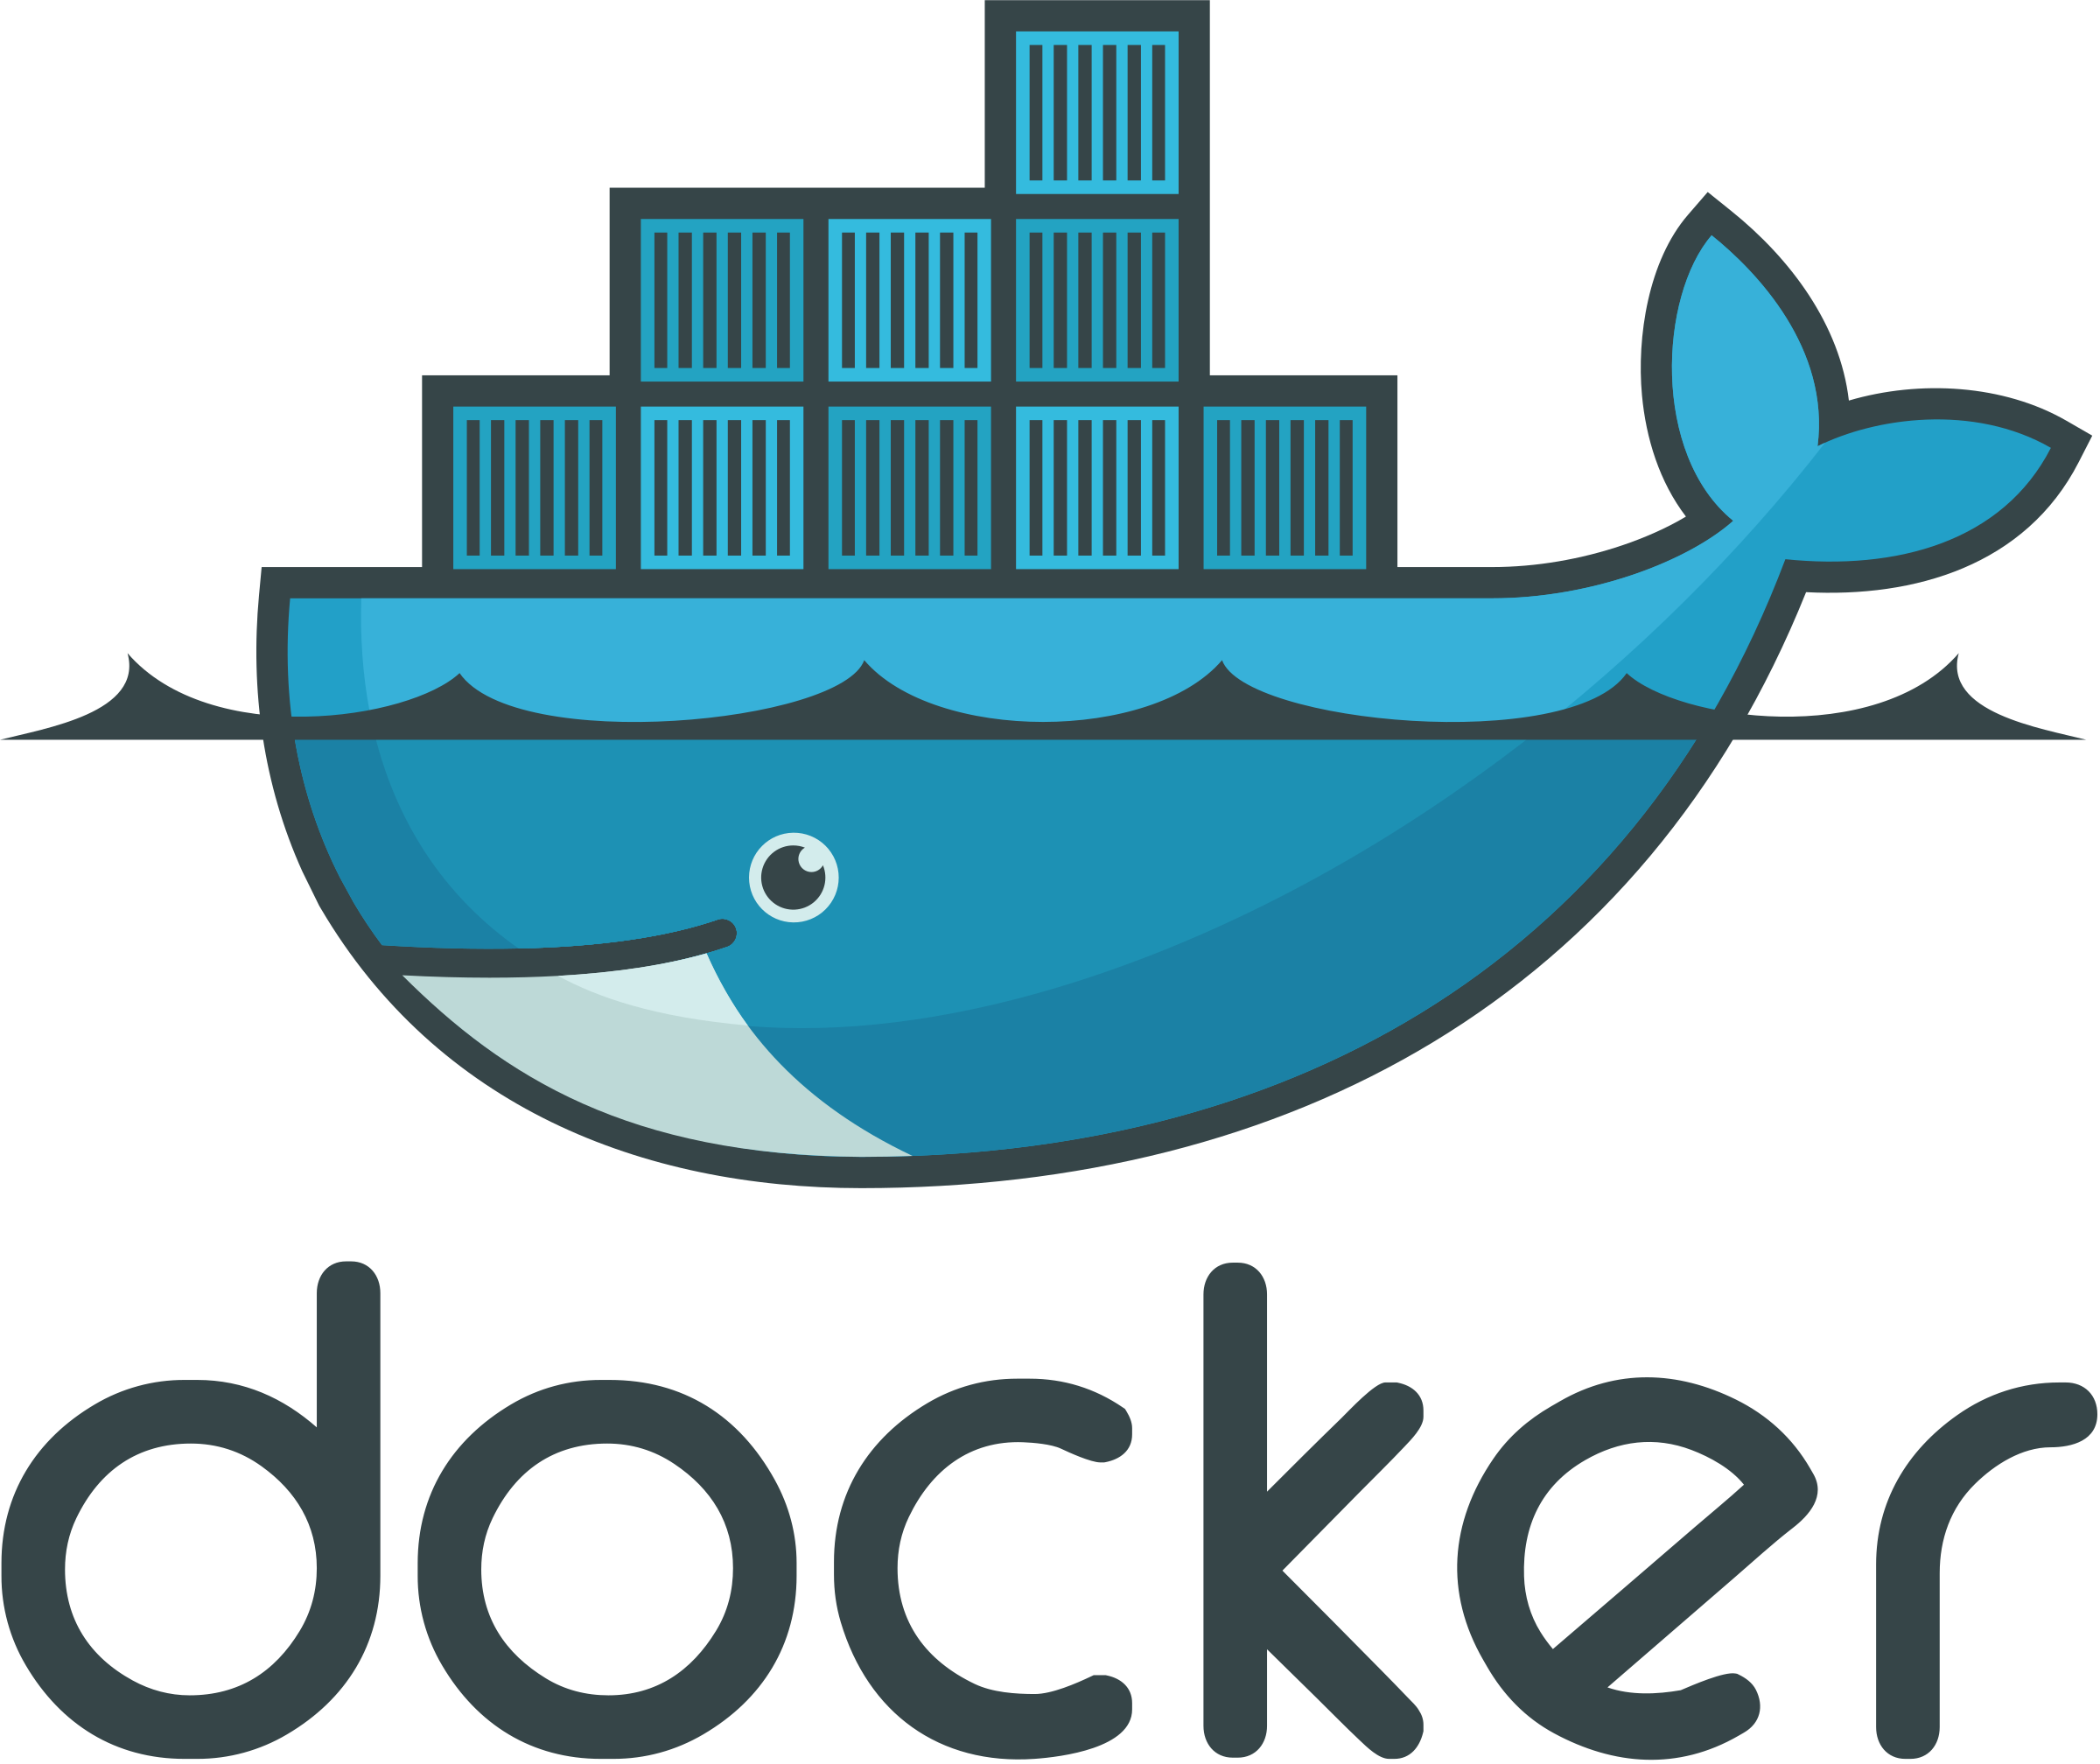
\includegraphics[width=1cm,height=1cm]{imgs/dockerLogo.png}
è un progetto open source che ha l'obiettivo di automatizzare il deployement dell'applicazione all'interno di un software container, fornendo un livello di astrazione superiore a quello del sistema operativo. 
L'idea alla base è avere un sistema di packaging uniforme che possa essere eseguito ovunque (architetture x86(\_64) e kernel linux). 
Il motivo per cui è utile docker è che lavora sul kernel linux ed è così indipendente dalla particolare distro e posso installarci delle librerie che in generale sarebbero in contrasto con le librerie del sistema.\\
Docker aderisce alle policy delle OCI e non è l'unico sistema a farlo, tutti i sistema che vi si aderiscono in teoria dovrebbero permettere l'interoperabilità.
Uno degli obiettivi principali è isolare le applicazioni, cioè voglio che non vedano i processi del sistema (per motivi di sicurezza). 
Inoltre sono lightweight poiché condividono il kernel di OS e non c'è uno strato di virtualizzazioni in mezzo.\\
L'idea è quella di eliminare hypervisor ed eliminare GuestOS, permettendo l'esecuzione delle applicazioni direttamente sul OS. 
La tecnologia container ha la dualità immagini - container, immagine è un file/template che contiene i meta data e configurazione e questo file viene usato per creare container, la differenza rispetto alle VM è che il container non è una copia dell'immagine (vedi AMI) bensì una sua esecuzione, un'altra differenza è il tempo di esecuzione rispetto alle VM che ci mettono tempi in ordini di minuti siccome docker è un processo parte in ordini di secondi.\\
Le immagini sono salvate di solito su Hub o registro locale.
Il \textbf{filesystem} di docker è solo di lettura ed è a livelli (UnionFS), creare l'immagine a livello permette la massima riusabilità delle immagini, si può ripartire a creare un immagine a partire da una già esistente, ad esempio se ho un'immagine debian con emacs sopra posso partire da debian e mettere sopra nano e per fare ciò non devo riscaricare debian posso riusare già l'immagine di debian che possiedo. Riesce a creare questo modello a strati seguendo un approccio Copy-on-Write, cioè crea una copia del file modificato. 
Tutte le tecnologie tranne il filesystem a strati sono dovute usando il kernel linux, uno di queste tecnologie è il \textbf{namespaces}: permette l'isolamento dei processi, individuando le cose che può e non può vedere il processo. 
l'altra tecnologia principale che permette l'esecuzione dei docker è \textbf{cgroups}: che ha lo scopo di limitare e monitorare l'accesso alle risorse(CPU, Memoria, I/O, network).\\
Docker è un demone linux che mostra un'interfaccia REST che è utilizzabile tramite una CLI (command line interface) fornita da docker.
\begin{figure}[!h]
	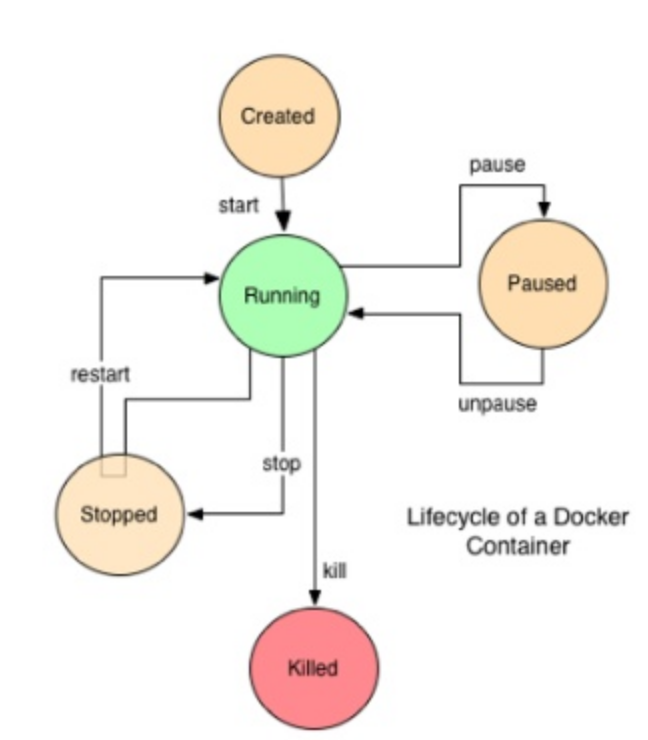
\includegraphics[width=\linewidth,height=7cm]{imgs/Docker_life.png}
	\caption{Ciclo di vita del Docker}
	\label{fig:dlife}
\end{figure}
Il ciclo di vita di un container è così come indicato in Figura \ref{fig:dlife} e i comandi principali sono:
\begin{myitemize}
	\item docker create: crea ma non esegue il docker
	\item docker run: crea ed esegue il docker
	\item docker stop
	\item docker start
	\item docker restart
	\item docker rm
	\item docker kill
\end{myitemize}
Essendo un processo come gli altri docker di default può vedere tutta le risorse che il computer ha a disposizione, è possibile limitare con dei soft limits (limite inferiore delle risorse) e hard limits (limite superiore) l'accesso a queste risorse.\\
Quando si elimina l'immagine in esecuzione si perdono tutti i dati, quindi nasce il concetto di volume che sono cartelle condivise con il sistema (per non perdere i dati).
I volumi sono di tre tipi:
\begin{myitemize}
	\item Bind Mount: è una cartella montata è in binding (collegata) a una cartella del sistema host;
	\item Volume Mount: sono anch'esse cartelle condivise ma gestiti dal docker, evitando problema di breech;
	\item tmpfs Mount: cartelle che non sono sul disco della macchina ma sulla memoria.
\end{myitemize}
Tutto questo modello dei volumi quando ci troviamo nel cloud non funziona possono esservi diversi errori (fallisce una VM) e il volume è esplicitamente al Host, per rendere la persistenza del volume anche nel cloud docker è stato scritto in una maniera da poter usare dei plugin, il plugin per lavorare in locale (quello che abbiamo visto) si chiama local persist, esistono diversi plugin già creati dai vari provider cloud per funzionare sul loro sistema.\\
Il building process del docker è l'output di un dockerfile che contiene le istruzioni per far partire e il contesto che sono una serie di altre informazioni necessarie.
Le istruzione sono sequenziali e vengono eseguite dal demone docker. Tra i comandi esistenti i più importanti sono:
\begin{itemize}[wide, noitemsep, topsep=0ex]
	\item \textbf{ENTRYPOINT}: definisce un processo che deve essere eseguita al lancio del container, può avere due forme:
	\begin{verbatim}
		ENTRYPOINT[``executable'', ``param1'',\ 
		           ``param2'']   (exec form)
		ENTRYPOINT executable param1\
		             param2      (shell form)
	\end{verbatim}
	La differenza è che la shell form viene comandato dalla shell quindi ad es. si può terminare un processo con ctrl+c.
	\item \textbf{CMD} ha lo stesso significato della ENTRYPOINT, ma ha una differenza, se esiste un già ENTRYPOINT viene eseguito ENTRYPOINT e CMD gli passa i suoi parametri e se esistono molteplici CMD viene eseguito l'ultimo CMD. Es:
	\begin{verbatim}
		CMD[``--port 27017'']
		ENTRYPOINT /usr/bin/mongod
		# ENTRYPOINT riceve il parametro da CMD
	\end{verbatim}
\end{itemize}
La comunicazione tra i vari container si fa attraverso il docker networking, che è una tecnologia di virtualizzazione della rete, i docker connessi credono di avere a disposizione una propria connessione, questa connessione è un plugin del docker, questa connessione è inoltre distribuita e decentralizzata quindi ogni docker ha una parte d'informazione della rete.
Questa idea viene formalizzata nel CNM (Container Network Model) che consiste di 4 elementi principali:
\begin{enumerate}[noitemsep, topsep=0ex]
	\item Sandbox: è una struttura che contiene le configurazioni della rete a livello di container, quindi gestisce le interfacce, la tabella di routing e una serie di informazioni del DNS. Una sandbox può avere più di un endpoint e collegata a più reti ma ogni container può essere collegato solo ad una Sandbox;
	\item Endpoint: è l'implementazione dell'interfaccia di rete (es. veth - Virtual Ethernet) Un endpoint può essere associato ad una sola rete e una sola sandbox;
	\item Network: è l'insieme di tanti endpoint che possono comunicare tra di loro;
	\item Cluster: l'insieme di docker collegati ad una rete.
\end{enumerate}
Quando creiamo una rete questa può essere di tipo:
\begin{myitemize}
	\item NULL: Il container non ha accesso alla rete;
	\item Host: Il container e l'host hanno la stessa interfaccia di rete;
	\item Bridge: E' un servizio a cui vari endpoint sono collegati;
	\item Overlay: Una rete che viene creata tra più host docker;
	\item Remote: E' un'interfaccia definita in modo tale da essere implementa da terze parti.
\end{myitemize}

\subsection{Docker-Compose}
E' un linguaggio dichiarativo esprimibile attraverso file yaml, che descrive com'è costruita un'applicazione multicontainer come la rete e volume.
In pratica usa i comandi docker dietro e semplifica la vita allo sviluppatore. Il file docker-compose.yml è composta da tre sezioni: Services, Networks e Volumes.\\
Un \textbf{Docker Swarm} è un cluster di macchine che usano docker e si uniscono logicamente in un sistema, ai fini di deployement è come se diventassero un'unica macchina.
Il cluster viene gestito non più dalle singole istanze di docker sulle macchine ma da una istanza sola che prende il nome di swarm manager, le altre macchine vengono chiamate worker (o nodes).
Il manager può usare diverse strategie per eseguire i container nei vari workers, un esempio è emptiest node dove i container vengono fatti partire nel nodo può vuoto.
Solo il manager può decidere di eseguire i comandi o autorizzare l'aggiunga nello swarm di altri worker, i worker quindi mettono a disposizione solo le risorse computazionali e ricevono ordini dal manager.\\
Le funzionalità di docker swarm:
\begin{myitemize}
	\item Gestione del Cluster integrata con docker-machine, non necessita di software aggiuntivi esterni;
	\item Modello di servizio dichiarativo;
	\item Gestione della scalabilità automatica, creando anche repliche di container e costantemente continua a controllare lo stato di vita dei workers;
	\item Riconciliazione dello stato attuale con lo stato dichiarato dall'utente;
	\item Gestione della multi host networking con reti overlay;
	\item Implementazione del servizio discovery per l'individuazione dei nodi in maniera unica;
	\item Load Balancing, in caso di esistenza di varie istanze dello stesso servizio, queste riceveranno il carico distribuito;
	\item Sicuro di default poiché i vari nodi comunicano attraverso protocolli http criptati utilizzando tecnologie TLS.
\end{myitemize}
Si possono avere più di un manager ma solo uno è leader gli altri sono detti Reachable e sono una sorta di leader di backup nel caso il leader fallisca ottenendo alta disponibilità, possono usare dei protocolli di consenso per prendere decisioni insieme.

\section{Serverless}
Esistono altri 2 modelli per il cloud oltre a IaaS, Paas e SaaS: \textbf{CaaS} (Container as a Service) e \textbf{FaaS} (Function as a Service).\\
Serverless può essere inteso come BaaS (Backend as a Service) oppure FaaS.
Il BaaS è l'incorporazione di servizi autonomi in modalità PaaS di un'applicazione ad esempio il servizio di autenticazione.
Nel FaaS lo sviluppatore non deve sviluppare applicazioni intere, ma solo scrivere delle funzioni che siano più semplici possibili, queste funzioni devono avere un ruolo atomico e granulare.
Sono dei container computazionali, che contengono una funzione effimera, che viene eseguita in caso di un evento esterno e queste funzioni sono gestite totalmente dal cloud provider.\\
In questo caso non vi è un gestione centralizzata, infatti preferisce la coreografia (coordinazione) delle funzione rispetto all'orchestrazione (non c'è un decisore centrale che richiama le funzioni), ottenendo così:
\begin{myitemize}
	\item Flessibilità e Estendibilità: si possono aggiungere altre funzioni senza alterare quelle pre-esistenti; 
	\item Divisione delle preoccupazione;
	\item Costo ridotto: Non si paga se la funzione non è in esecuzione, quindi se una funzione è raramente usata non pago un server costantemente accesso.
\end{myitemize}
Inoltre non sono più vincolato solo dai linguaggi offerti dal cloud provider, qualunque linguaggio che compila su un processo UNIX (quindi nel docker) va bene.
Vi sono dei contraints, ad esempio in AWS una funzione può al massimo durare 5 minuti, se una funzione richiede più di 5 minuti forse conviene prendere un IaaS o PaaS, oppure si possono splittare le funzioni in più funzioni.
Inoltre non vi è la garanzia del fatto che gli stati persistano su invocazioni multiple successive poiché le variabili sono salvati su memoria o un disco locale.\\
Le funzioni in FaaS sono tipicamente triggerate da eventi definiti dal cloud provider ad es. AWS include aggiornamenti sul S3, task schedulati, ricezioni di messaggi in un servizio di coda (come Kafka) oppure per le rispondere alle richieste HTTP che usano API Gateway.\\
Un altro svantaggio è il così detto cold start - crea una nuova istanza, inizia le funzioni host ecc. e il periodo di accensione dipende dal linguaggio di programmazione, le librerie da caricare e la configurazione della funzione e la quantità di codice, pur essendo in ordini di secondi è molto lento rispetto a warm start, che riusa una istanza di Lambda function esistente da una chiamata precedente.\\
I benefici sono molteplici:
\begin{myitemize}
	\item Costi Operazionali, di Sviluppo e Esecuzione Ridotti;
	\item Computazione più \textcolor{OliveGreen}{\textbf{Green}} ed efficiente.
\end{myitemize}
Vi sono anche dei svantaggi:
\begin{myitemize}
	\item Il controllo del Vendor: I downtime, i limiti, cambiamenti di costo, aggiornamenti di API;
	\item Problemi di mantenimento;
	\item La durata di esecuzione;
	\item Latenza di inizializzazione;
	\item Testing, Debugging e monitoraggio difficile e limitato.
\end{myitemize}
Quindi il serverless è non ottimale per le funzioni che hanno bisogno di stati e sono più lunghe in generale ad es. Deep Learning Training, Streaming Pesante, Analitiche Hadoop, Gestione DB, streaming video ecc. Sono molto utili per eventi veloci, stateless e event-driven come microservizi, IoT, Inferenze ML, streaming leggero ecc.

\section{Apache Spark}
L'idea di fondo non è quella di spostare i dati nelle varie macchine ma i codici (data locality), quindi una volta ottenuto il parallelismo e data locality e in più implementiamo un sistema che sia in grado di gestire i fallimenti a vari livelli allora otteniamo il framework chiamato Hadoop.
Spark piano piano sta sostituendo una parte dell'ecosistema di Hadoop.\\
Per introdurre il concetto degli operatori serve capire cos'è il linguaggio funzionale: è un paradigma di programmazione, che vede la computazione come processo di valutazioni di funzioni matematiche, queste funzioni devono essere immutabili e prive di stato. 
Le proprietà della programmazione funzionale:
\begin{myitemize}
	\item Composizione di funzioni per ottenere funzione di ordine superiore
	\item Le funzioni sono senza stato (sono pure), prendono stato grazie ad un accumulatore che è una variabile passata in ingresso a una funzione
	\item Non possono modificare lo stato di altri funzioni (no side-effect)
	\item Possibilità di Ricorsione
	\item Lazy-Evaluation, esecuzione solo quando viene veramente richiesta
	\item Le funzioni non modificano le strutture dati, ma ne creano altre durante il processo
\end{myitemize}
Grazie a queste proprietà si ottiene la parallelizzazione automatica, performance migliorata, nessun Bug e gestione della memoria.\\
I due operatori più interessanti per Spark sono:
\begin{myitemize}
	\item \textbf{Map}: un operatore di ordine superiore, prende in ingresso una funzione e una input list e applica questa funzione in ingresso a tutti gli elementi della input list restituendo un'altra lista;
	\item \textbf{Reduce}: un operatore di ordine superiore, prende in ingresso una funzione e una input list e applica questa funzione ricorsivamente a tutti gli elementi restituendo una combinazione della lista.
\end{myitemize}
\subsection{MapReduce}
Una loro applicazione combinata è MapReduce, che serve a processare una grande quantità di dati con algoritmi parallelizzati e distribuiti su un cluster. 
Il sistema shuffla i dati nelle fasi in mezzo a Map e Reduce. 
I nodi del sistema condividono un filesystem distribuito e vengono sfruttati nelle due fasi:
\begin{myitemize}
	\item Fase \textbf{Map}: Il master node partiziona i files in M splits attraverso una chiave, e assegna ai slaves i maps da eseguire.\\
	Questi slaves dopo aver eseguito il task di Map, scrivono il loro output sul disco partizionato in R regioni attraverso una funzione hash;
	\item Ad altri slaves viene assegnato il task \textbf{Reduce}, ciascuna slave legge i dati dal disco del mapper corrispondente e li raggruppano in base alla chiave ed eseguono la funzione di Reduce.
\end{myitemize}
Questo è l'architettura usata in Hadoop 1.x, uno dei suoi svantaggi sono il blocco che si crea ai vari slaves, poiché quando lavorano i Mapper i Reducer sono fermi e quando lavorano i Reducer i Mapper sono quelli fermi, quindi non si sfrutta la massima capacità del cluster. In Hadoop 2.x e Spark si è cercato di colmare questa problematica. 
Un altro svantaggio è che ad ogni iterazione di Map e Reduce il file viene scritto sul disco che rallenta tutto il processo. 
Inoltre non tutti lavori possono essere scritti in alberi di operazioni Map e Reduce, ad es. i cicli sui dati stessi.\\
\subsection{Spark Ecosystem}
Qua entra in gioco un'applicazione open source 
\includegraphics[width=1cm,height=0.6cm]{imgs/sparkLogo.png}: esso effettua i calcoli in memoria senza riscriverli sul disco se non necessario e permette di generalizzare i calcoli usando grafi aciclici ottenendo molta più flessibilità. Allarga il set delle operazioni da solo Map e Reduce in \textbf{trasformazioni} e \textbf{azioni}, dove trasformazioni e azioni sono un set di operazioni diverse che possono essere combinate in maniera arbitraria e Spark 2 ha implementato anche un ottimizzatore di query (Catalyst). \\
Apache Spark supporta:
\begin{myitemize}
	\item Manipolare i dati attraverso SQL, vedendo i file come delle tabelle SQL;
	\item Esiste una libreria MLlib per Data Science e Machine Learnig distribuito;
	\item Processamento di grafi di dimensioni enormi;
	\item Processamento di dati in tempo reale;
	\item File system Distribuito in-memory(cache);
	\item Query approssimate sui dati;
	\item Eredita da Hadoop il supporto dei file Avro, Parquet e le sorgenti di questi dati possono essere HDFS, Cassandra, Hive, Mongo ecc.;
	\item Sviluppo in linguaggi come Python, R, Scala, Java, .Net;
\end{myitemize}
\begin{figure}
	\centering
	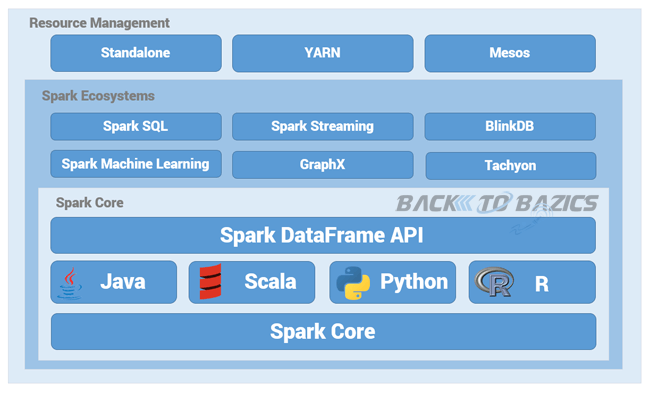
\includegraphics[width=\linewidth]{imgs/Spark_eco.png}
	\caption{Spark Ecosystem}
	\label{fig:SparkEco}
\end{figure}
Al centro di tutto l'ecosistema c'è il Spark Core che si occupa di:
\begin{myitemize}
	\item Gestione del calcolo distribuito, quindi si occupa della distribuzione, coordinamento e scheduling dei task computazionali e inoltre si occupa di gestire i fallimenti e riduce al minimo la data shuffling tra i vari nodi;
	\item Fornire le API per l'astrazione delle \textbf{RDD}, che è un collezione di oggetti, immutabili e fault tollerant partizionati su un cluster, che possono essere manipolati in parallelo.
\end{myitemize}
Spark può essere deployato in 3 modalità diverse:
\begin{myenumerate}
	\item Come una libreria che viene eseguita in un programma, fornendo le API delle RDD, ma si possono usare solo le risorse della macchina su cui gira il programma;
	\item Può essere eseguito in maniera distribuita (su cluster), che può essere standalone (che non significa solo una macchina ma semplicemente il fatto che non ha bisogno di un scheduler esterno) oppure usando scheduler esterni tra cui YARN, Mesos e K8;
	\item In modalità MR, in questo caso l'accesso ai sistemi di storage attraverso le API di Hadoop per usare HBase, S3, Cassandra ecc.
\end{myenumerate}
L'applicazioni Spark ha due elementi fondamentali più un terzo facoltativo:
\begin{myenumerate}
	\item \textbf{Spark Driver} che è la parte del codice che viene eseguita non in parallelo, questo driver crea uno SparkContext per gestire i jobs, lo SparkContext deve capire quali pezzi del nostro codice sono parallelizzabile e deve inviarli al cluster;
	\item Nei vari cluster ci sono degli agenti \textbf{Executor} che eseguono gli ordini dal SparkContext e riescono a gestire una serie di task in parallelo, una volta concluso il task il risultato viene ri-inviato al driver;
	\item Nel mezzo può esserci un \textbf{Cluster Manager} per permettere la comunicazione tra il driver e i vari nodi e di allocare le risorse.
\end{myenumerate}
Il context era un oggetto che creava delle connessioni ad es. per connettere SQL si creava SQLContext, per connettere Hive si creata HiveContext, ciò creava confusione e rendeva difficile una loro collaborazione. 
Questi diversi contesti, in Spark 2, vengono unificati in un unico oggetto chiamato SparkSession, ottenendo un entrypoint unificato per gestire i dati in spark.
\subsection{RDD}
RDD (Resilient Distributed Dataset), essenzialmente una lista di oggetti distribuita e resiliente, distribuita nel senso che sono partizionati (in base a una chiave) in memoria di vari nodi ma viene vista come un'unica lista grazie alla chiave di partizionamento ciascuna partizione contiene un unico record che può essere operato indipendentemente (simile all'approccio Shared Nothing), ciò permettere la loro gestione in maniera parallela con le trasformazioni (Map, Filter) e in caso di fallimento vengono automaticamente ricostruiti.\\
Vengono di solito immagazzinati in memoria ma vi è la possibilità di scriverli sul disco, sono tipizzati (Integer, double, Objects), sono immutabili (quindi applicare una trasformazione significa creare un altro RDD) e sono lazy evaluated. Alcune possibili trasformazioni sono: map, filter, union, intersection, distinct e join (solo per RDD di tipo key-value).\\
Ciascun RDD tiene traccia delle trasformazioni usate per costruirlo, questa traccia è detta lineage, che può essere usato per ricostruire i dati persi. 
Le Action possono prendere un RDD e produrre un altro oggetto non RDD. 
Le trasformazioni sono lazy e non vengono eseguite finché non c'è un azione su RDD che li convoca. \\
Il Driver pianifica l'ordine di esecuzione convertendo le trasformazioni e azioni in un grafo aciclico diretto (DAG), queste DAG tracciano le dipendenze (Lineage) e i nodi del grafo sono RDD mentre gli archi rappresentano le trasformazioni.
Le azioni sono il pezzo finale del grafo e triggerano l'esecuzione della DAG, un'azione per esempio può essere reduce, count, collect, save.\\
Attenzione se io devo effettuare due azioni sullo stesso DAG, le trasformazioni del DAG vengono eseguite 2 volte, per evitare tale problema si può inserire il comando cache prima dell'esecuzione delle azioni. 
Alcune trasformazioni, come sortByKey, join, groupByKey ecc., possono avere uno shuffle che può rallentare il sistema, le trasformazioni possono essere:
\begin{myitemize}
	\item Narrow dependency: Ciascuna RDD viene consumato da al più una partizione figlio ma un figlio può avere molteplici genitori, quindi non cambia il numero di partizioni tra una trasformazione e l'altra, e non avviene lo shuffle;
	\item Wide dependency: Ciascun RDD può essere usato da molteplici partizioni figli, quindi cambia il numero di partizioni
\end{myitemize}
Spark fa questa distinzione perché eseguirà le operazione Narrow tutte insieme in parallelo, spark divide in lavoro in stage, in base alla presenza di operazioni shuffle, all'interno di ciascun stage le operazioni possono essere eseguite in parallelo, inoltre le trasformazioni nei vari stage vengono composte per velocizzare il tutto.\\
I vantaggi di RDD sono il controllo a basso livello, grazie alle API, su cosa fa spark e sono inoltre typesafe: spark ci permette di fare operazioni in base al tipo di RDD e infine ci insegnano in profondità come funzione spark.\\
I suoi svantaggi sono il fatto che sono difficile da gestire (per un data scientist che deve usare i DataFrames), inoltre cambia la velocità di esecuzione anche in base al linguaggio usato (usando Java/Scala si ottiene un boost di performance anche 2x rispetto a python) e infine l'ottimizzazione del codice non avviene e quindi programmi sono meno efficienti.\\
\subsection{Spark SQL}
E' una libreria che funziona su Spark Core e fornisce come astrazione del RDD il dataframe, con tutte le proprietà dei dataframe, sono delle tabelle con righe e colonne con i header e indici ecc.
A questo punto si può usare la tecnologia molto sviluppata dei database SQL, Spark SQL ha implementato anche un ottimizzatore che viene usato da tanti motori SQL.
Questo aumenta anche il supporto alle varie tipologie di file e sorgenti con cui spark può comunicare.\\
I Dataframe essendo un'astrazione delle RDD hanno le sue proprietà: sono immutabili, distribuiti, rappresentano una collezione, sono lazyily evaluated e le azioni sono eagerly evaluated.\\
Il risultato di usare i dataframe è non solo la stessa velocità indipendentemente dal linguaggio scelto ma addirittura un miglioramento rispetto a lavorare direttamente su RDD, questo anche perché i DataFrame sono compressi quindi usano meno memoria, inoltre viene tenuto in conto anche l'inefficienza dei programmatori mediamente parlando.

\section{Stream Processing}
La differenza tra il batch processing e stream processing è:
\paragraph{Batch Processing} lavora su batch di dati limitati ottenuti da un data store e il risultato è un altro batch di dati. Batch ha accesso a tutti i dati, si può lavorare a qualcosa di grande e complesso, la latenza è misurata in minuti, di solito uno è interessato all'output (qualità) di dati che alla latenza.
\paragraph{Stream Processing} lavora su un flusso continuo (infinito) di dati, il risultato è un nuovo stream di dati e per ciò è dovuto al fatto che il processo stream non finisce. La funzione in questo caso è applicata ad un datapoint o una finestra piccola di dati recenti, inoltre la computazione deve essere leggera poiché lo stream deve continuare ad andare e la latenza deve essere near real time o al più secondi.\\
Gli elementi principali di un'applicazione stream sono:
\begin{myenumerate}
	\item Sorgente: che produce i dati in input;
	\item Trasformazioni: prende l'input del dataflow e producono alcuni output;
	\item Sink: riceve/consuma i dati dell'output delle trasformazioni;
	\item Data Pipeline: è una sequenza di trasformazioni, rappresentate di solito da un grafo aciclico diretto;
	\item Event/Tuple/message: E' l'elemento atomico del data flow (come una riga di un dataframe).
\end{myenumerate}
Generalmente i sistemi di stream di dati sono generalmente distribuiti, per gestire più dati in parallelo e quindi con maggiore velocità, ma avvolte vi sono delle operazioni sequenziali e si fa fatica a renderli distribuiti. I dati in ingresso possono essere partizionati e ciascuna operatore può eseguirsi in una maniera concorrente. Ottiene le proprietà dei sistemi distribuiti tra quali: Fault-tollerance, Load Balancing.\\
Lo stato dello streaming può essere molto utile, ad esempio per riconoscere qualche pattern negli eventi o per aggregazioni di dati, e lo stato di fault tolerance viene gestito in utilizzando i due meccanismi di \textbf{Checkpoint and Replay}: salvataggio periodico dello stato dell'operatore su un storage sicuro (es. HDFS), in caso di fallimento tutti i dati dopo l'ultimo checkpoint dovranno essere rianalizzati (Replay).\\
Nel caso di dati ``illimitati'' in streaming di solito si preferisce usare il windowing per tagliare i dati dando a loro il senso temporale. Queste finestre possono essere:
\begin{myitemize}
	\item Fixed (Tumbling) window es. calcolo di qualcosa ogni tot unità temporale
	\item Sliding window es. calcola di qualcosa in un unità temporale ogni tot unità temporale (possibilmente diversa da quella del calcolo)
	\item Sessione window, la sessione è definita come il periodo di attività terminato da un periodo di inattività più grande di una certa soglia, quindi sono finestre dinamiche e sono totalmente data driven, anzi sono molto compatibili con un sistema distribuito e ciascuna partizione avrà la sua finestra.
\end{myitemize}
Esistono anche altri metodi di approssimazione, oltre a windowing, per gestire dati illimitati ad es. sampling con streaming K-means ecc., essendo delle approssimazioni vi sono degli errori. 
In generale sono algoritmi molto complessi poiché devono anche garantire un limitate superiore degli errori.\\
\textbf{SQL on Streams} consiste nel vedere uno stream di dati come una tabella relazionale di dimensione infinita, a questo punto si può usare SQL per generare un'analisi o trasformazione, il sistema ci mostra una tabella (dinamica) ma sotto ha un sistema di streaming distribuito che genera a partire da uno streaming in entrata uno streaming in uscita.

\subsection{Apache Storm}

\includegraphics[width=1.5cm,height=0.5cm]{imgs/stormLogo.png} è disegnato per supportare lo stream di applicazioni e supporta fino ad 1 milione di messaggi al secondo, può scalare a miglia di nodi per cluster ed è fault tollerant e usando strumenti di terze parti, in particolare Trident è in grado di applicare anche la semantica temporale ``exactly once''.\\
Il modello concettuale è un modello molto semplice ed include:
\begin{myitemize}
	\item Tupla: è l'unità core (il messaggio) e può essere vista come una coppia chiave valore;
	\item Stream: è la sequenza infinità delle tuple;
	\item Spout: è la sorgente dello stream e il suo compito è quelli di emettere delle tuple;
	\item Bolt: riceve le tuple, fa una certa computazione (può anche leggere e scrivere dati da uno store) ed opzionalmente emette altre tuple.
\end{myitemize}
La topologia è un DAG di spouts e bolts, nella quale ciascun spout/bolt esegue solo un task, quindi durante la definizione della topologia bisogna specificare come i spout e bolt sono tra loro collegati, il partizionamento dei dati dello stream fra i bolt è detto \textbf{stream grouping}, i vari tipi di stream grouping sono:
\begin{myitemize}
	\item Shuffle: il partizionamento è randomico, i spout mandano in maniera randomica i dati verso i bolts a cui sono collegati;
	\item Fields: il partizionamento è basato su un campo della tupla, può essere utile ad esempio nel conteggio di tuple con un certo valore in un campo;
	\item All: ciascun bolt riceve una istanza di una tupla;
	\item Custom;
	\item Direct: già la sorgente decide a quale bolt mandare la tupla;
	\item Global: Tutte le tuple generate da tutte le istanze di una sorgente vengono mandate a un unico target.
\end{myitemize}
Il cluster totale è gestito da Nimbus che calcola gli assignment e li invia allo ZooKeeper e lo ZooKeeper li invia ai vari supervisori sui vari cluster che scaricano la topologia da Nimbus, questa topologia viene mandata in esecuzione attraverso un processo Java. 
Lo ZooKeeper si preoccupa anche di controllare la salute dei vari nodi con HeartBeat e se un Worker muore, il supervisore lo riavvia e se continua a morire Nimbus assegna il worker (che può contenere più di un operatore) a un altro supervisor, mentre se muore tutto il nodo il lavoro viene assegnato ad un altro nodo. Se dovesse morire Nimbus, i supervisor continuano a lavorare ma il riassegnamento diventa impossibile, quindi conviene mettere Nimbus con alta disponibilità (magari tenerne uno di backup), mentre Zookeeper è fault tollerant per se.\\
I processi che garantiscono l'affidabilità (ad es. che una tupla venga per forza vista) sono:
\begin{myitemize}
	\item Ack and Fail: Ciascuna tupla generata ha un unico ID e ciascuna tupla processata deve essere ackata e fallita, in caso di processamento completato viene generato un ack e fail in caso di timeout, il messaggio viene tracciato da un task detto ``acker'' in caso di fallimento lo spout può far ripartire il messaggio se è programmato in tale modo;
	\item Anchoring: Un bolt può emettere una nuova tupla ancorata alla tupla input, quindi nel caso del fallimento lo spout tuple alla radice del DAG andrà rieseguito.
	%domanda ^ ma Anchoring allora a cosa serve se deve far ripartire tutto?
\end{myitemize}
Esiste una libreria esterna Trident che permette di scrivere ad alto livello anche architetture molto complesse, mentre rimane stateful senza che sia l'utente a basso livello a definirla, permette di lavorare al livello micro batch, cioè non lavora ogni singolo messaggio che gli arriva ma accorpa un numero di messaggi, questo migliora il throughput ma peggiora la latenza.
Riesce a passare da at least one di storm a exactly once.

\subsection{Spark Streaming}
Spark è fatto per funzionare con l'idea del batch, per implementare lo streaming sfrutta il così detto mini-batch, quindi si aumenta la latenza ma si alza anche il thoughput. 
Spark streaming quindi porta con sé tutte le proprietà già esistenti in spark tra cui: distributività, disponibilità e scalabilità.
Il funzionamento inizia con i receiver che ricevono e emettono batch che in spark diventano RDD.\\
Grazie a spark streaming la creazione di un'architettura lambda avviene non solo nello stesso linguaggio ma addirittura nello stesso programma.\\
Alla base di spark ci sono gli RDD che possono essere distribuiti e replicati in memoria, quindi in caso di un problema di un nodo non perdo i dati, e grazie alla lineage posso anche capire da quale punto si dovrebbe far ripartire la computazione (a differenza di storm che deve far ripartire tutto).
I minibatch discretizzati RDD si chiamano \textbf{Dstreams}, la loro misura è fatta in modo da avere una latenza di circa 1 secondo e hanno un potenziale di potersi combinare con i batch proccessing.
Inoltre con la funzione union è stato possibile implementare il concetto di finestra.\\
Il master continua a salvare gli stati dei Dstream in un file checkpoint e in caso di fallimento del master questo può essere reinizializzato a partire da questo file checkpoint, permettendo un recupero rapido.\\
I Dstream richiedono una buona conoscenza di programmazione, quindi si è creata una sua astrazione sotto il nome di Spark Structured Streaming, che ha delle API a livello più alto rispetto a Dstreams.
I Dstreams mostrano lo streaming come delle tabelle dinamiche, mentre le operazioni vengono eseguite incrementalmente, quindi il risultato è un altro dataframe con dati variabili nel tempo.
L'analisi dei dati provenienti dal Output mode viene eseguita in base a un trigger: che può essere una funzione della sessione temporale.

\subsection{Amazon Big Data}
Amazon è il leader nel cloud computing, e offre un sacco di servizi direttamente lui pronti spesso anche per la scalabilità quindi non vi è neanche il bisogno di configurarli o mantenerli, e se un servizio non è direttamente offerto, è molto probabile che venga offerto nel marketplace. \\
La Big Data pipeline è costituita a un livello alto da:
\begin{myitemize}
	\item Data Ingestion/Data collection;
	\item Data Storage;
	\item Processare e analizzare i data;
	\item Consumare o visualizzare.
\end{myitemize}
e il suo obiettivo è minimizzare la latenza e il costo e massimizzare il throughput, nel cloud cerco di minimizzare la latenza ad esempio raggruppando le macchine vicine e inoltre massimizzo il thorughput grazie alla scalabilità dello storage e tutte le macchine leggono alla stessa velocità quindi la velocità di lettura cresce linearmente col crescere dei nodi e per quanto riguarda i costi essi vengono minimizzati poiché pago solo ciò che uso.
Il problema rimane il passaggio totale al cloud, ad esempio perché può essere costoso trasmettere tutti i dati, oppure potrebbero esserci problemi di privacy, esistono anche degli approcci ibridi in cui è possibile usare il proprio cloud per dati privati e Amazon per dati normali.\\
Lo stream storage di amazon è possibile con: Apache Kafka (esiste una cosa simile anche in amazon detta Amazon MQ), Amazon Kinesis e Amazon DynamoDB (simile a SQL streaming di spark). 
I file storage offerti possono essere HDFS, S3 e Amazon Glacier, sono tutte e tre supportati da Big Data Framework e sono altamente disponibili, la scelta avviene se i dati sono caldi (vengono acceduti molte volte) qua conviene usare HDFS o se sono freddi (pochi accessi) qua conviene Glacier, mentre S3 è una via di mezzo. Infine per i database e search engines abbiamo: Amazon ElastiCache, DynamoDB, RDS e ES.

\begin{figure}
	\centering
	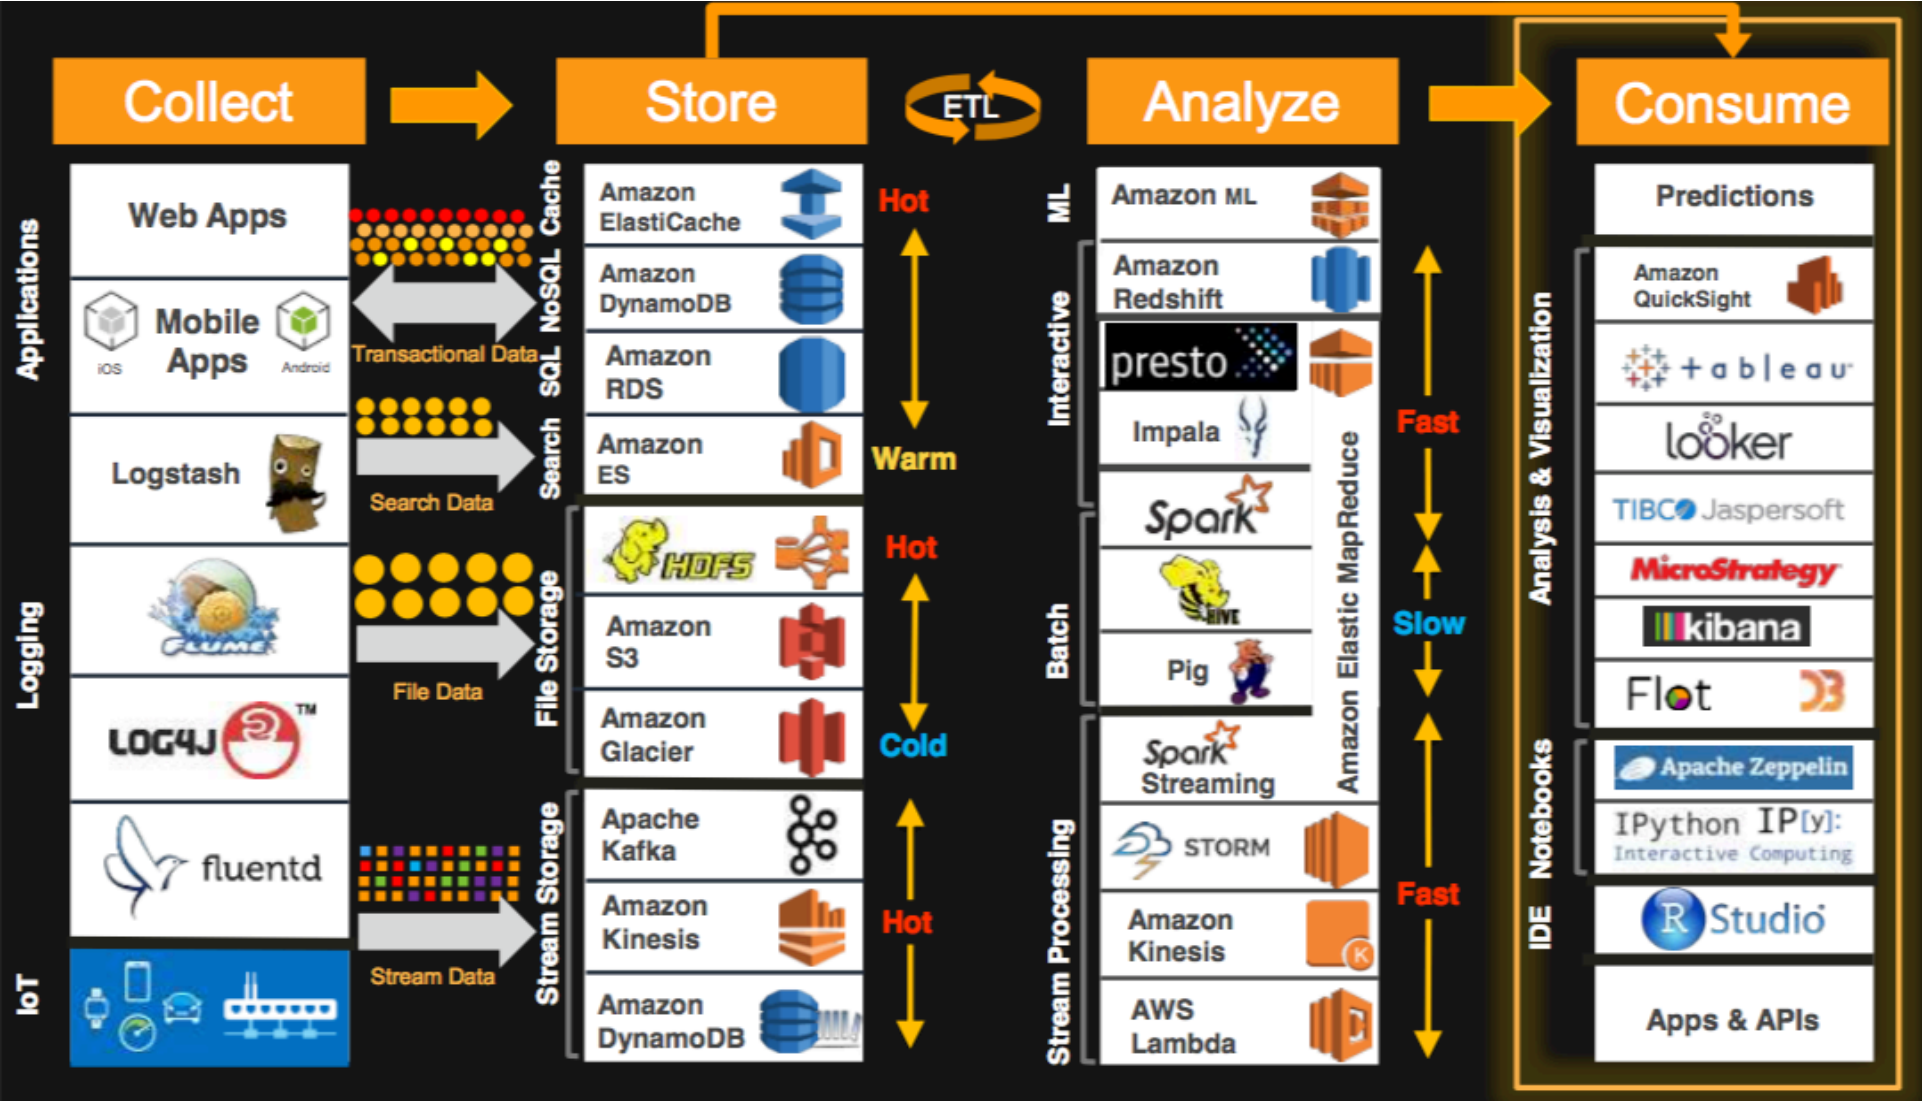
\includegraphics[width=\linewidth,height=7cm]{imgs/amazon_insight.png}
	\caption{Insight of the Amazon Services}
	\label{fig:amazon}
\end{figure}

\newpage

\part*{Part II - Prof Melen}


\end{document}